\newpage
\section{Hai mặt phẳng song song}
\subsection{LÝ THUYẾT CẦN NHỚ}
\subsubsection{Định nghĩa hai mặt phẳng song song}
\begin{itemize}
	\item Cho hai mặt phẳng $(P)$ và $(Q)$, có thể xảy ra một trong ba trường hợp
	\immini{
	\textbf{- Trường hợp 1:} $(P)$ và $(Q)$ có ba điểm chung không thẳng hàng, ta nói hai mặt phẳng $(P)$ và $(Q)$ trùng nhau, kí hiệu $(P)\equiv(Q)$.}{
		\begin{tikzpicture}[scale=0.8, font=\footnotesize, line join=round, line cap=round, >=stealth]
			\coordinate (M) at (0,0);
			\coordinate (N) at (2,2);
			\coordinate	(P) at (6,2);
			\coordinate	(Q) at (4,0);
			\coordinate	(A) at (2,1); \draw[fill=black] (A) node[left]{$A$} circle(1pt);
			\coordinate	(B) at (3,0.5); \draw[fill=black] (B) node[below]{$B$} circle(1pt);
			\coordinate	(C) at (3.5,1.5); \draw[fill=black] (C) node[right]{$C$} circle(1pt);
			\draw (M)--(N)--(P)--(Q)--(M);
			\draw pic[draw,blue,angle radius=7mm,angle eccentricity=1.5] {angle = Q--M--N};
			\draw pic[draw,blue,angle radius=7mm,angle eccentricity=1.5] {angle = N--P--Q};
			\draw (0.5,-0.1) node[above] {$P$};
			\draw (5.5,2.1) node[below] {$Q$};
		\end{tikzpicture}}
\immini{\textbf{- Trường hợp 2:} $(P)$ và $(Q)$ phân biệt và có một điểm chung, ta nói $(P)$ và $(Q)$ cắt nhau theo giao tuyến $d$ đi qua điểm chung, kí hiệu $(P)\cap(Q)=d$.}
	{\begin{tikzpicture}[scale=0.5, font=\footnotesize, line join=round, line cap=round, >=stealth]
			\coordinate (M) at (0,0);
			\coordinate (N) at (2,2);
			\coordinate	(P) at (9,2);
			\coordinate	(Q) at (7,0);
			\coordinate (A) at (3,3);
			\coordinate (B) at (5,5);
			\coordinate	(C) at (6,-1);
			\coordinate	(D) at (4,-3);
			\coordinate	(I) at (7/2,0);
			\coordinate	(J) at (11/2,2);
			\coordinate	(G) at (19/6,2);
			\coordinate	(H) at (35/6,0);
			\coordinate	(K) at (9/2,1);
			\draw (G)--(N)--(M)--(Q)--(P)--(J)--(B)--(A)--(D)--(C)--(H) (I)--(J);
			\draw[dashed] (G)--(J)--(H);
			\draw pic[draw,blue,angle radius=7mm,angle eccentricity=1.5] {angle = Q--M--N};
			\draw pic[draw,blue,angle radius=7mm,angle eccentricity=1.5] {angle = C--D--A};
			\draw (0.8,-0.1) node[above] {$P$};
			\draw (4.3,-2.7) node[above] {$Q$};
			\draw (3.8,0.3) node[right] {$d$};
			\draw[fill=black] (K) node[right]{$M$} circle(1pt);
		\end{tikzpicture}}
\immini{\textbf{- Trường hợp 3:} $(P)$ và $(Q)$ không có bất kì điểm chung nào, nghĩa là $(P)\cap(Q)=\varnothing$, ta nói $(P)$ và $(Q)$ song song với nhau, kí hiệu $(P)\parallel(Q)$ hoặc $(Q)\parallel(P)$.
}{	\begin{tikzpicture}[scale=0.5, font=\footnotesize, line join=round, line cap=round, >=stealth]
			\coordinate (M) at (0,0);
			\coordinate (N) at (2,2);
			\coordinate	(P) at (6,2);
			\coordinate	(Q) at (4,0);
			\coordinate (A) at (0,2.5);
			\coordinate (B) at (2,4.5);
			\coordinate	(C) at (6,4.5);
			\coordinate	(D) at (4,2.5);
			\draw (M)--(N)--(P)--(Q)--(M);
			\draw (A)--(B)--(C)--(D)--(A);
			\draw pic[draw,blue,angle radius=7mm,angle eccentricity=1.5] {angle = Q--M--N};
			\draw pic[draw,blue,angle radius=7mm,angle eccentricity=1.5] {angle = D--A--B};
			\draw (0.8,-0.1) node[above] {$P$};
			\draw (0.9,2.4) node[above] {$Q$};
		\end{tikzpicture}}
\begin{dn} Hai mặt phẳng được gọi là \textbf{\textit{song song}} nếu chúng không có điểm chung.
		\end{dn}
\end{itemize}
\subsubsection{Điều kiện để hai mặt phẳng song song}
\begin{dl} \immini{Nếu mặt phẳng $(P)$ chứa hai đường thẳng $a,b$ cắt nhau và hai đường thẳng đó cùng song song với mặt phẳng $(Q)$ thì $(P)$ song song với $(Q)$.\\
Tóm tắt $$\heva{&a,\,b\subset (P)\\&a\,\text{và}\,b\,\text{cắt nhau} 
	\\
	&a \parallel (Q) \;  \\&b \parallel (Q) 
} \Rightarrow (P) \parallel (Q).$$	

}{
		\begin{tikzpicture}[scale=0.7, font=\footnotesize, line join=round, line cap=round, >=stealth]
			\coordinate (M) at (0,0);
			\coordinate (N) at (2,2);
			\coordinate	(P) at (6,2);
			\coordinate	(Q) at (4,0);
			\coordinate (A) at (0,2.5);
			\coordinate (B) at (2,4.5);
			\coordinate	(C) at (6,4.5);
			\coordinate	(D) at (4,2.5);
			\coordinate	(U) at (1.8,2.8);
			\coordinate	(V) at (5.0,4.2);
			\coordinate	(S) at (2.3,4.2);
			\coordinate	(T) at (3.7,2.8);
			\draw (M)--(N)--(P)--(Q)--(M);
			\draw (A)--(B)--(C)--(D)--(A) (U)--(V) (S)--(T);
			\draw pic[draw,blue,angle radius=7mm,angle eccentricity=1.5] {angle = Q--M--N};
			\draw pic[draw,blue,angle radius=7mm,angle eccentricity=1.5] {angle = D--A--B};
			\draw (0.6,-0.1) node[above] {$Q$};
			\draw (0.6,2.4) node[above] {$P$};
			\draw (U) node[above] {$a$};
			\draw (T) node[above] {$b$};
		\end{tikzpicture}}
\end{dl}
\begin{hq}
Nếu mặt phẳng $(P)$ chứa hai đường thẳng $a$, $b$ cắt nhau và hai đường thẳng đó lần lượt song song với hai đường thẳng $c$, $d$ nằm trong mặt phẳng $(Q)$ thì $(P)$ song song với $(Q)$.\\
	\immini{Tóm tắt
		 $$\heva{&a,\,b\subset (P)\\&a\,\text{và}\,b\,\text{cắt nhau} 
			\\
			&a \parallel c\;  \\&b \parallel d\\&c,\,d\subset (Q) 
		} \Rightarrow (P) \parallel (Q).$$	}{\begin{tikzpicture}[>=stealth,x=1cm,y=1cm,scale=.8,font=\footnotesize]
			\coordinate (A) at (-4,-2);
			\coordinate (B) at (0,-2);
			\coordinate (C) at (1,0);
			\coordinate (D) at (-3,0);
			\draw(A)--(B)--(C)--(D)--cycle;
			\fill (-1.5,2) circle (1.0pt) node[above]{$I$};
			\draw (-3,2) node[above]{$a$};
			\draw (-2.5,2.5) node[above]{$b$};
			\draw (-3,-1) node[above]{$c$};
			\draw (-2.5,- 0.5) node[above]{$d$};
			\draw(A)--(B)--(C)--(D)--cycle;
			\coordinate(A1) at (-4,1);
			\coordinate (B1) at (0,1);
			\coordinate (C1) at (1,3);
			\coordinate (D1) at (-3,3);
			\draw (-3,2)--(0,2) (-2.5,2.5)--(-.5,1.5) (-3,-1)--(0,-1) (-2.5,-0.5)--(-.5,-1.5) ;
			\draw pic[draw,angle radius=7mm,angle eccentricity=0.65,"$Q$"] {angle = B--A--D};
			\draw pic[draw,angle radius=7mm,angle eccentricity=0.65,"$P$"] {angle = B1--A1--D1};
			\draw(A1)--(B1)--(C1)--(D1)--cycle;
	\end{tikzpicture}}
	\end{hq}
\subsubsection{Tính chất của hai mặt phẳng song song}
\begin{dl}
\immini{Qua một điểm nằm ngoài một mặt phẳng cho trước có một và chỉ một mặt phẳng song song với mặt phẳng đó.}{
		\begin{tikzpicture}[scale=0.7, font=\footnotesize, line join=round, line cap=round, >=stealth]
			\coordinate (M) at (0,0);
			\coordinate (N) at (2,2);
			\coordinate	(P) at (6,2);
			\coordinate	(Q) at (4,0);
			\coordinate (A) at (0,2.5);
			\coordinate (B) at (2,4.5);
			\coordinate	(C) at (6,4.5);
			\coordinate	(D) at (4,2.5);
			\coordinate	(I) at (1.8,0.3);
			\coordinate	(J) at (5.0,1.7);
			\coordinate	(G) at (2.3,1.7);
			\coordinate	(H) at (3.7,0.3);
			\coordinate	(U) at (1.8,2.8);
			\coordinate	(V) at (5.0,4.2);
			\coordinate	(S) at (2.3,4.2);
			\coordinate	(T) at (3.7,2.8);
			\draw (M)--(N)--(P)--(Q)--(M);
			\draw (A)--(B)--(C)--(D)--(A)
			% (I)--(J) (G)--(H) %(U)--(V) (S)--(T)
			;
			\draw pic[draw,blue,angle radius=7mm,angle eccentricity=1.5] {angle = Q--M--N};
			\draw pic[draw,blue,angle radius=7mm,angle eccentricity=1.5] {angle = D--A--B};
			\draw (0.6,-0.1) node[above] {$Q$};
			\draw (0.6,2.4) node[above] {$P$};
%			\draw (I) node[above] {$a'$};
%			\draw (U) node[above] {$a$};
%			\draw (H) node[above] {$b'$};
%			\draw (T) node[above] {$b$};
			\fill (3,3.5) circle(1pt) node[below]{$A$};
		\end{tikzpicture}}
\end{dl}
\begin{dl}
	\immini{
	 Cho hai mặt phẳng $(P)$ và $(Q)$ song song với nhau. Nếu $(R)$ cắt $(P)$ thì cắt $(Q)$ và hai giao tuyến của chúng song song với nhau.\\
 Tóm tắt
 $$\heva{&(P) \parallel (Q)
 	\\& (R)\cap (P)=a} \Rightarrow \heva{& (R)\cap (Q)=b
 \\
 &a \parallel b.
}$$

}{
		\begin{tikzpicture}[scale=0.5, font=\footnotesize, line join=round, line cap=round, >=stealth]
			\coordinate (A) at (0,0);
			\coordinate (B) at (3,2);
			\coordinate	(C) at (10,2);
			\coordinate	(D) at (7,0);
			\coordinate (M) at (0,-3);
			\coordinate (N) at (3,-1);
			\coordinate	(P) at (10,-1);
			\coordinate	(Q) at (7,-3);
			\coordinate	(U) at (4,3);
			\coordinate	(V) at (7,5);
			\coordinate	(S) at (8,-4);
			\coordinate	(T) at (5,-6);
			\coordinate	(I) at (37/9,2);
			\coordinate	(J) at (13/3,0);
			\coordinate	(K) at (40/9,-1);
			\coordinate	(L) at (14/3,-3);
			\coordinate	(E) at (22/3,2);
			\coordinate	(F) at (218/29,10/29);
			\coordinate	(G) at (23/3,-1);
			\coordinate	(H) at (227/29,-71/29);
			\draw (J)--(A)--(B)--(I)--(J) (E)--(C)--(D)--(J)--(E) (M)--(N)--(K)--(L)--(M);
			\draw (L)--(G)--(P)--(Q)--(L) (H)--(S)--(T)--(U)--(V)--(E) (F)--(G);
			\draw[dashed] (I)--(E)--(F) (K)--(G)--(H);
			\draw pic[draw,blue,angle radius=8mm,angle eccentricity=1.5] {angle = Q--M--N};
			\draw pic[draw,blue,angle radius=8mm,angle eccentricity=1.5] {angle = D--A--B};
			\draw pic[draw,blue,angle radius=6mm,angle eccentricity=1.5] {angle = S--T--U};
			\draw (1.2,-0.1) node[above] {$P$};
			\draw (1.2,-3.2) node[above] {$Q$};
			\draw (5.35,-5.8) node[above] {$R$};
			\draw (5,1) node[right] {$a$};
			\draw (5,-2) node[right] {$b$};
		\end{tikzpicture}}	
\end{dl}
	\subsubsection{Định lý Thalès trong không gian}
\begin{dl} Ba mặt phẳng đôi một song song chắn trên hai cát tuyến bất kì các đoạn thẳng tương ứng tỉ lệ.
\end{dl}
\immini
{Cho ba mặt phẳng $(P)$, $(Q)$, $(R)$ đôi một song song và hai đường thẳng $d$, $d'$. Đường thẳng $d$ cắt $(P)$, $(Q)$, $(R)$ theo thứ tự tại $A$, $B$, $C$, thẳng $d'$ cắt $(P)$, $(Q)$, $(R)$ theo thứ tự tại $A'$, $B'$, $C'$. Khi đó, ta có $$\dfrac{AB}{A'B'}= \dfrac{BC}{B'C'}= \dfrac{AC}{A'C'}.$$
}
{
	\begin{tikzpicture}[>=stealth,line join=round,line cap=round,font=\footnotesize,scale=0.8]
		\path
		(4,0) coordinate (uq)
		(3.2,0) coordinate (up)
		(4.8,0) coordinate (ur)
		(1,1.4) coordinate (vq)
		(0.8,1.2) coordinate (vp)
		(1.2,1.5) coordinate (vr)
		(0,0) coordinate (q)
		(0.75,2) coordinate (p)
		(-0.75,-2) coordinate (r)
		($(q)+(uq)$) coordinate (q1)
		($(q)+(vq)$) coordinate (q2)
		($(q1)+(q2)-(q)$) coordinate (q3)
		($(p)+(up)$) coordinate (p1)
		($(p)+(vp)$) coordinate (p2)
		($(p1)+(p2)-(p)$) coordinate (p3)
		($(r)+(ur)$) coordinate (r1)
		($(r)+(vr)$) coordinate (r2)
		($(r1)+(r2)-(r)$) coordinate (r3)
		(2.5,4) coordinate (x)
		(1,-3) coordinate (x4)
		(3,4) coordinate (y)
		(4,-3) coordinate (y4)
		(intersection of x--x4 and p--p1) coordinate (x1) 
		(intersection of x--x4 and q--q1) coordinate (x2) 
		(intersection of x--x4 and r--r1) coordinate (x3) 
		(intersection of y--y4 and p--p1) coordinate (y1) 
		(intersection of y--y4 and q--q1) coordinate (y2) 
		(intersection of y--y4 and r--r1) coordinate (y3) 
		($(x)!.7!(x1)$) coordinate (A)
		($(x)!.81!(x2)$) coordinate (B)
		($(x)!.8!(x3)$) coordinate (C)
		($(y)!.6!(y1)$) coordinate (A')
		($(y)!.85!(y2)$) coordinate (B')
		($(y)!.93!(y3)$) coordinate (C')
		;
		\draw 
		(p)--(p1)--(p3)--(p2)--cycle
		(q)--(q1)--(q3)--(q2)--cycle
		(r)--(r1)--(r3)--(r2)--cycle
		(x)--(A) (x1)--(B) (x2)--(C) (x3)--(x4)
		(y)--(A') (y1)--(B') (y2)--(C') (y3)--(y4)
		(A)--(A') (B)--(B') (C)--(C')
		;
		\draw[dashed] 
		(A)--(x1) (B)--(x2) (C)--(x3)
		(A')--(y1) (B')--(y2) (C')--(y3)
		;
		\begin{scope}
			\clip (q1)--(q)--(q2);
			\draw (q) circle (.8cm);
			\draw ($(q)+(30:.5cm)$) node{$Q$};
		\end{scope}
		\begin{scope}
			\clip (p1)--(p)--(p2);
			\draw (p) circle (.8cm);
			\draw ($(p)+(30:.5cm)$) node{$P$};
		\end{scope}
		\begin{scope}
			\clip (r1)--(r)--(r2);
			\draw (r) circle (.8cm);
			\draw ($(r)+(30:.5cm)$) node{$R$};
		\end{scope}
		\foreach \p/\g in {A/180, B/180, C/180, A'/0, B'/0, C'/0}
		\draw[fill=black] (\p) circle (1pt) node[shift=(\g:3mm)] {$\p$};
		\draw (x) node[below left] {$d$};
		\draw (y) node[below right] {$d'$};
\end{tikzpicture}}
	\subsubsection{Hình lăng trụ và hình hộp}
\begin{enumerate}[1)]
	\immini{	\item \textbf{Hình lăng trụ}. Cho hai mặt phẳng $(P)$ và $\left(P'\right)$ song song với nhau. Trên $(P)$ cho đa giác lồi $A_1 A_2 \ldots A_n$. Qua các đỉnh của đa giác này, ta vẽ các đường thẳng song song với nhau và cắt $\left(P'\right)$ lần lượt tại $A_1'$, $A_2'$, $\ldots$, $A_n'$. Hình tạo bởi các hình bình hành $A_1 A_2 A_2' A_1'$, $A_2 A_3 A_3' A_2'$, $\ldots$, $A_n A_1 A_1' A_n'$ và hai đa giác $A_1 A_2 \ldots A_n$, $A_1' A_2' \ldots A_n'$ gọi là hình lăng trụ, kí hiệu $A_1 A_2 \ldots A_n \cdot A_1' A_2' \ldots A_n'$.\\
		Trong hình lăng trụ $A_1 A_2 \ldots A_n$, $A_1' A_2' \ldots A_n'$, ta gọi
		\begin{itemize}
			\item Hai đa giác $A_1 A_2 \ldots A_n$ và $A_1' A_2' \ldots A_n'$ là hai \textbf{mặt đáy} nằm trên hai mặt phẳng song song.
			\item Các điểm $A_1$, $A_2$, $\ldots$, $A_n$, $A_1'$, $A_2'$, $\ldots$, $A_n'$ là các \textbf{đỉnh}.
			\item Các hình bình hành $A_1 A_2 A_2' A_1'$, $A_2 A_3 A_3' A_2'$, $\ldots$, $A_n A_1 A_1' A_n'$ là các \textbf{mặt bên}.
			\item Các đoạn thẳng $A_1 A_1'$, $A_2 A_2', \ldots, A_n A_n'$ là các \textbf{cạnh bên}.
			\item Các cạnh bên song song và bằng nhau.
			\item Các cạnh của hai đa giác đáy là các \textbf{cạnh đáy}. Các cạnh đáy tương ứng song song và bằng nhau.
		\end{itemize}
	}
	{	    \begin{tikzpicture}[font=\footnotesize,yscale=0.9]
			\coordinate (A) at (0,0);
			\coordinate (B) at (5.5,0);
			\coordinate (C) at (6.5,2);
			\coordinate (A1) at (0,4.5);
			\coordinate (M1) at (1,7);
			\coordinate (N1) at (2,-1);
			\coordinate (D) at ($(C)-(B)+(A)$);
			\coordinate (B1) at ($(B)-(A)+(A1)$);
			\coordinate (C1) at ($(C)-(B)+(B1)$);
			\coordinate (D1) at ($(C1)-(B1)+(A1)$);
			\coordinate (A11) at ($(M1)!.78!(N1)$);
			\coordinate[shift={(1,-0.3)}] (M2) at (1,7);
			\coordinate[shift={(3,-0.2)}] (M3) at (1,7);
			\coordinate[shift={(3.5,0.5)}] (M4) at (1,7);
			\coordinate[shift={(1.5,0.7)}] (M5) at (1,7);
			\coordinate[shift={(1,-0.3)}] (N2) at (2,-1);
			\coordinate[shift={(3,-0.2)}] (N3) at (2,-1);
			\coordinate[shift={(3.5,0.5)}] (N4) at (2,-1);
			\coordinate[shift={(1.5,0.7)}] (N5) at (2,-1);
			\coordinate[shift={(1,-0.3)}] (B11) at ($(M1)!.78!(N1)$);
			\coordinate[shift={(3,-0.2)}] (C11) at ($(M1)!.78!(N1)$);
			\coordinate[shift={(3.5,0.5)}] (D11) at ($(M1)!.78!(N1)$);
			\coordinate[shift={(1.5,0.7)}] (E11) at ($(M1)!.78!(N1)$);
			\coordinate (A22) at ($(M1)!.22!(N1)$);
			\coordinate[shift={(1,-0.3)}] (B22) at ($(M1)!.22!(N1)$);
			\coordinate[shift={(3,-0.2)}] (C22) at ($(M1)!.22!(N1)$);
			\coordinate[shift={(3.5,0.5)}] (D22) at ($(M1)!.22!(N1)$);
			\coordinate[shift={(1.5,0.7)}] (E22) at ($(M1)!.22!(N1)$);
			\path[name path=k1] (M1)--(N1); 
			\path[name path=k2] (M2)--(N2);
			\path[name path=k3] (M3)--(N3);
			\path[name path=k4] (M4)--(N4);
			\path[name path=k5] (M5)--(N5);
			\path[name path=ab] (A)--(B); 
			\path[name path=cd] (C)--(D);
			\path[name path=a1b1] (A1)--(B1);
			\path[name intersections={of=k1 and ab,by=E1}];
			\path[name intersections={of=k2 and ab,by=E2}];
			\path[name intersections={of=k3 and ab,by=E3}];
			\path[name intersections={of=k4 and ab,by=E4}];
			\path[name intersections={of=k5 and ab,by=E5}];
			\path[name intersections={of=k1 and cd,by=F1}];
			\path[name intersections={of=k4 and cd,by=F4}];
			\path[name intersections={of=k1 and a1b1,by=G1}];
			\path[name intersections={of=k2 and a1b1,by=G2}];
			\path[name intersections={of=k3 and a1b1,by=G3}];
			\path[name intersections={of=k4 and a1b1,by=G4}];
			\path[name intersections={of=k5 and a1b1,by=G5}];
			\draw (M1)--(A22) (M2)--(B22) (M3)--(C22) (M4)--(D22) (M5)--(E22);
			\draw (F1)--(D)--(A)--(B)--(C)--(F4) (A1)--(B1)--(C1)--(D1)--cycle (A11)--(G1) (B11)--(G2) (C11)--(G3) (D11)--(G4) (E1)--(N1) (E2)--(N2) (E3)--(N3) (E4)--(N4) (E5)--(N5) (A11)--(B11)--(C11)--(D11) (A22)--(B22)--(C22)--(D22)--(E22)--cycle;
			\draw[dashed] (A11)--(E1) (B11)--(E2) (C11)--(E3) (D11)--(E4) (E11)--(E5) (F1)--(F4) (A22)--(G1) (B22)--(G2) (C22)--(G3) (D22)--(G4) (E22)--(E11) (A11)--(E11)--(D11);
			\draw (A11) node[left] {$A_1$} (A22) node[left] {$A_1'$} (B11) node[below left] {$A_2$} (C11) node[below left] {$A_3$} (D11) node[right] {$A_4$} (E11) node[above left] {$A_5$} (B22) node[below left] {$A_2'$} (C22) node[below left] {$A_3'$} (D22) node[right] {$A_4'$} (E22) node[below left] {$A_5'$};
			%		\draw pic[draw,"$P'$"]{angle=B--A--D} pic[draw,"$P$"]{angle=B1--A1--D1};
	\end{tikzpicture}}
	\textbf{Chú ý:} Hình lăng trụ có đáy là tam giác, tứ giác, ngũ giác,$\ldots$ tương ứng được gọi là hình lăng trụ tam giác, hình lăng trụ tứ giác, hình lăng trụ ngũ giác,$\ldots$
			\item \textbf{Hình hộp}.  Hình hộp là hình lăng trụ có đáy là hình bình hành.\\
	Trong một hình hộp ta có
	\immini{
		\begin{itemize}
			\item Sáu mặt là sáu hình bình hành. Mỗi mặt đều có một mặt song song với nó.
			\item Hai mặt như thế gọi là hai mặt đối diện.
			\item Đoạn thẳng nối hai đỉnh đối diện gọi là đường chéo.
			\item Bốn đường chéo cắt nhau tại trung điểm của mỗi đường.
		\end{itemize}
	}
	{\begin{tikzpicture}[scale=0.6, font=\footnotesize, line join=round, line cap=round, >=stealth]
			\path
			(0,0)coordinate(A)
			(-2,-2)coordinate(B)
			(6,0)coordinate(D)
			($(B)+(D)-(A)$)coordinate(C)
			($(A)+(1,5)$)coordinate(A')
			($(A')+(B)-(A)$)coordinate(B')
			($(A')+(C)-(A)$)coordinate(C')
			($(A')+(D)-(A)$)coordinate(D')
			;
			\coordinate (I) at ($(A)!0.5!(C')$);
			\draw(B)--(B') (C)--(C') (D)--(D') (B)--(C)--(D) (A')--(B')--(C')--(D')--(A') ;
			\draw[dashed](B)--(A)--(D) (A)--(A') (D)--(B') (C)--(A') (B)--(D') (A)--(C');
			\foreach \p/\q in {A/-180, B/-90, C/-90, D/0, A'/90, B'/-180, C'/90, D'/90, I/-90} \fill[black] (\p) circle (1pt) ($(\p)+(\q:2.5mm)$) node{$\p$};
	\end{tikzpicture}}
\end{enumerate}
\subsection{PHÂN LOẠI VÀ PHƯƠNG PHÁP GIẢI TOÁN}
\begin{dang}{Chứng minh hai mặt phẳng song song}
\end{dang}
\setcounter{vd}{0}
\begin{vd}%[1H4H4-2]%[Dự án đề cương 3 khối NH24-25-Dot2-Huỳnh Đức Vũ]
	Cho hình chóp $S.ABCD$ có đáy là hình thang $ABCD$ đáy lớn $AD$ và $AD=2BC$. Gọi $M$ và $N$ lần lượt là trung điểm của $SA$ và $AD$. Chứng minh rằng hai mặt phẳng $(BMN)$ và $(SCD)$ song song với nhau.
	\loigiai{\immini{
		Ta có
		\begin{itemize}
		\item
		 $MN$ là đường trung bình của $\triangle SAD$ nên $MN\parallel SD$.
\item 	$\heva{&MN \parallel SD\\&
		MN\not \subset (SCD)}\Rightarrow MN\parallel (SCD)$.
	\end{itemize}
	Tương tự, ta có tứ giác $BCDN$ có $BC\parallel ND$ và $BC=ND$ nên là hình bình hành. Suy ra $BN\parallel CD$, do đó $BN\parallel (SCD)$. \\
	Vì $MN \parallel (SCD)$ và $BN \parallel (SCD)$, đồng thời hai đường thẳng $MN$, $BN$  cùng nằm trong mặt phẳng $(BMN)$ và cắt nhau tại $N$ nên $(BMN)\parallel(SCD)$.
	}{	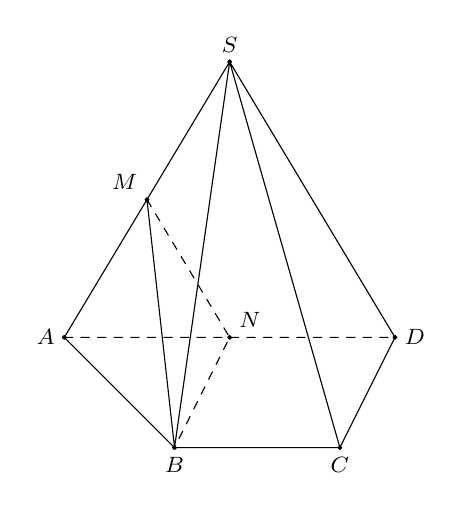
\begin{tikzpicture}[scale=0.7, font=\footnotesize, line join=round, line cap=round, >=stealth]
		\coordinate (A) at (0,0);
		\coordinate (B) at (2,-2);
		\coordinate	(C) at (5,-2);
		\coordinate	(D) at (6,0);
		\coordinate (S) at (3,5);
		\coordinate (M) at (1.5,2.5);
		\coordinate	(N) at (3,0);
		\draw (S)--(A)--(B)--(C)--(D)--(S)--(C) (S)--(B) (M)--(B);
		\draw[dashed] (M)--(N)--(B) (A)--(D);
		\draw[fill=black] (A) node[left]{$A$} circle(1pt);
		\draw[fill=black] (B) node[below]{$B$} circle(1pt);
		\draw[fill=black] (C) node[below]{$C$} circle(1pt);
		\draw[fill=black] (D) node[right]{$D$} circle(1pt);
		\draw[fill=black] (S) node[above]{$S$} circle(1pt);
		\draw[fill=black] (M) node[above left]{$M$} circle(1pt);
		\draw[fill=black] (N) node[above right]{$N$} circle(1pt);
\end{tikzpicture}}}
\end{vd}
\begin{vd}%[1H4H4-2]%[Dự án đề cương 3 khối NH24-25-Dot2-Huỳnh Đức Vũ]
	Cho tứ diện $ABCD$. Lấy $G_1$, $G_2$, $G_3$ lần lượt là trọng tâm của các tam giác $ABC$, $ACD$, $ADB$. Chứng minh rằng $\left(G_1 G_2 G_3\right) \parallel (B C D)$.
	\loigiai{\immini{Gọi $M$, $N$, $P$ lần lượt là trung điểm của $BC$, $CD$, $B D$.\\	
			Vì $M \in A G_1$ và $\dfrac{A G_1}{A M}=\dfrac{2}{3} ; N \in A G_2$ và $\dfrac{A G_2}{A N}=\dfrac{2}{3}$ nên $\dfrac{A G_1}{A M}=\dfrac{A G_2}{A N}$. Suy ra $G_1 G_2 \parallel M N$.\\
			Mà $M N \subset(B C D)$, $G_1 G_2  \not \subset(B C D)$ nên $G_1 G_2 \parallel(B C D)$.\qquad(1)\\
			Chứng minh tương tự ta cũng có $G_2 G_3 \parallel(B C D)$.\qquad(2)\\
			Vì $G_1 G_2$, $G_2 G_3$ nằm trong mặt phẳng $\left(G_1 G_2 G_3\right)$ và cắt nhau nên từ (1) và (2) ta có $\left(G_1 G_2 G_3\right) \parallel(B C D)$.}{\begin{tikzpicture}[scale=0.8, font=\footnotesize, line join=round, line cap=round, >=stealth]
				\coordinate[label=left:$B$] (B) at (0,0);
				\coordinate[label=right:$D$] (D) at (7,0);
				\coordinate[label=below:$C$] (C) at (3.5,-2);
				\coordinate (K) at ($(C)!0.5!(D)$);		
				\coordinate (O) at ($(B)!0.4!(K)$);
				\coordinate[label=above:$A$] (A) at ($(O)+(0,4)$);
				\coordinate[label=below:$M$] (M) at ($(B)!0.5!(C)$);
				\coordinate[label=below:$N$] (N) at ($(D)!0.5!(C)$);
				\coordinate[label=below:$P$] (P) at ($(B)!0.5!(D)$);
				\coordinate[label=left:$G_1$] (G1) at ($(A)!2/3!(M)$);
				\coordinate[label=right:$G_2$] (G2) at ($(A)!2/3!(N)$);
				\coordinate[label=right :$G_3$] (G3) at ($(A)!2/3!(P)$);
				\draw (A)--(B)--(C)--(D)--cycle (A)--(C) (A)--(M) (A)--(N);
				\draw [dashed] (B)--(D) (M)--(N)--(P)--cycle (G1)--(G2)--(G3)--cycle (A)--(P);
				\foreach \x in{A,B,C,D,M,N,P,G1,G2,G3} \draw[fill=black] (\x) circle (1pt);
	\end{tikzpicture}}}
\end{vd}
\begin{vd}%[1H4H4-2]%[Dự án đề cương 3 khối NH24-25-Dot2-Huỳnh Đức Vũ]
	Cho hai hình bình hành $ABCD$ và $ABEF$ ở trong hai mặt phẳng khác nhau. Trên các đường chéo $AC$ và $BF$ lần lượt lấy các điểm $M$, $N$ sao cho $AM = BN$. Các đường thẳng song song với $AB$ vẽ từ $M$, $N$ lần lượt cắt $AD$, $AF$ tại $M'$, $N'$.
	\begin{enumerate}
		\item Chứng minh $\left(BCE\right) \parallel \left(ADF\right)$.
		\item Chứng minh $\left(DEF\right)\parallel\left(MNN'M'\right)$.
	\end{enumerate}
	\loigiai{
	\immini{	\begin{enumerate}
			\item Vì $\heva{&BC\parallel AD\\&BE\parallel AF\\&BC\,\text{cắt nhau}}$ nên $\left(BCE\right)\parallel\left(ADF\right)$.
			\item Vì $\dfrac{AM}{AC} = \dfrac{BN}{BF} = \dfrac{AN'}{AF}$ nên $MN'\parallel CF$.\\
			Mặt khác, lại có $EF\parallel NN'$ (do cùng song song với $AB$) và hai đường thẳng $CE$, $EF$ cắt nhau nên ta có $\left(DEF\right)\parallel\left(MNN'M'\right)$.
		\end{enumerate}}{
	\begin{tikzpicture}[scale=.8, font=\footnotesize, line join=round, line cap=round, >=stealth]
	\path
	(2,2) coordinate (A)
	(0,0) coordinate (B)
	(5,-1) coordinate (C)
	(7,1) coordinate (D)
	(1,5) coordinate (E)
	(3,7) coordinate (F)
	(3,1) coordinate (M)
	(0.86,2) coordinate (N)
	(3.67,1.67) coordinate (M')
	(2.29,3.43) coordinate (N')
	;
	\draw (B)--(C)--(D)--(F)--(E)--(B) (C)--(E);
	\draw[dashed] (C)--(A)--(F) (D)--(A)--(B)--(F) (M)--(M')--(N')--(N)--(M);
	\foreach \x/\g in{A/60, B/-120, C/-60, D/0, E/90, F/90, M/-120, N/150, M'/40, N'/20}
	\fill[black](\x)circle(1pt)($(\x)+(\g:3mm)$)node{$\x$};
	\draw[fill=red,opacity=.1](M)--(M')--(N')--(N)--(M);
\end{tikzpicture}}
	}
\end{vd}

\begin{dang}{Chứng minh đường thẳng song song với mặt phẳng}
	\textbf{Phương pháp}.\\
	Để chứng minh đường thẳng $d$ song song với mặt phẳng $(P)$, ta chứng minh đường thẳng $d$ nằm trong một mặt phẳng $(Q)$ mà $(Q)$ song song với $(P)$.
\end{dang}
\setcounter{vd}{0}
	\begin{vd}%[1H4H4-2]%[Dự án đề cương 3 khối NH24-25-Dot2-Huỳnh Đức Vũ]
	Cho hình chóp $S.ABCD$, đáy $ABCD$ là hình bình hành có $O$ là giao điểm của hai đường chéo. Gọi $M, N$ lần lượt là trung điểm của $SA, SD$.
	\begin{itemize}
		\item[a)] Chứng minh rằng $(OMN) \parallel (SBC)$.
		\item[b)] Gọi $E$ là trung điểm của $AB$ và $F$ là một điểm thuộc $ON$. Chứng minh $EF$ song song với $(SBC)$.
	\end{itemize}
	\loigiai{
		\immini{	\begin{enumerate}[a)]
				\item Do $O M$ là đường trung bình của $\triangle S A C$ nên $O M \parallel S C. \qquad (1)$\\
				Lại có, $O N$ là đường trung bình của $\triangle S D B$ nên $O N \parallel S B. \qquad (2)$\\
				Từ $(1)$ và $(2)$ suy ra $(O M N) \parallel (S B C)$.
				\item Ta có $O E$ là đường trung bình của tam giác $A B D$ nên $O E \parallel A D$, mà $A D \parallel M N$, suy ra $O E \parallel M N$. Do đó $E$ thuộc mặt phẳng $(O M N)$.\\ Suy ra $EF \subset(O M N)$.\\ Theo ý a, ta có $(O M N) \parallel (S B C)$ nên $EF \parallel (S B C)$.
		\end{enumerate}}
		{	\begin{tikzpicture}[smooth,line join=round,line cap=round,font=\scriptsize,scale=0.7]
				\path 
				(0,0) coordinate (A)
				($(A)+(-135:3)$) coordinate (D)
				($(A)+(0:5)$) coordinate (B)
				($(B)+(D)-(A)$) coordinate (C)
				($(A)!0.5!(C)$) coordinate (O)
				($(O)+(90:5)$) coordinate (S);
				\coordinate (M) at ($(S)!0.5!(A)$);
				\coordinate (N) at ($(S)!0.5!(D)$);
				\coordinate (E) at ($(A)!0.5!(B)$);
				\coordinate (F) at ($(O)!0.65!(N)$);
				\draw [dashed] (S)--(A)--(D)--(B)--(A)--(C) (S)--(O) (O)--(N)--(M)--(E)--(O) (E)--(F);
				\draw (S)--(D)--(C)--(S)--(B)--(C);
				\foreach \x/\g in {A/180,D/180,C/0,B/0,O/-90,S/90, M/-360, N/-175, E/90, F/70}
				\fill[black] (\x) circle (1pt) + (\g:3mm) node {$\x$};
		\end{tikzpicture}}
	}
\end{vd}
\begin{vd}%[1H4H4-2]%[Dự án đề cương 3 khối NH24-25-Dot2-Huỳnh Đức Vũ]
	Cho hình chóp $S.ABCD$ có đáy $ABCD$ là hình bình hành. Gọi $G_1$, $G_2$, $G_3$ lần lượt là trọng tâm các tam giác $SAB$, $ABC$, $SBD$. Gọi $M$ là một điểm thuộc đường thẳng $G_2 G_3$. Chứng minh $G_1M \parallel (SBD)$.
	\loigiai{
	\immini{	
		Gọi $O$ là tâm hình bình hành $ABCD$ và $N$ là trung điểm $AB$, suy ra $G_1 \in SN$, $G_2 \in CM$, $G_3 \in SO$.
		Do $G_1$, $G_2$ lần lượt là trọng tâm các tam giác $SAB$, $ABC$ nên ta có 
		$$\dfrac{NG_1}{NS}=\dfrac{NG_2}{NC}=\dfrac{1}{3}\Rightarrow G_1G_2 \parallel SC \Rightarrow G_1G_2 \parallel (SBC).\qquad (1)$$
		Do $G_2$, $G_3$ lần lượt là trọng tâm tam giác $ABC$, $SBD$ nên 
			$$	\dfrac{OG_2}{OB}=\dfrac{OG_3}{OS}=\dfrac{1}{3}	
		\Rightarrow G_2G_3 \parallel SB
\Rightarrow G_2G_3 \parallel (SBC).\qquad (2$$
Từ $(1)$ và $(2)$ ta có $ (G_1G_2G_3) \parallel (SBC)$. \\
				Mà $G_1M \subset (G_1G_2G_3)$  nên $G_1M \parallel (SBC)$.
	}{\begin{tikzpicture}[scale=0.6]
		 \coordinate (A) at (3,3);
		\coordinate (B) at (0,0);
		\coordinate (C) at (8,0);
		\coordinate (D) at (11,3);
		\coordinate (S) at (3,10);
		 \coordinate (O) at ($0.5*(B) + 0.5*(D)$); % Trung điểm BD
		\coordinate (N) at ($0.5*(B) + 0.5*(A)$); % Trung điểm BA
		\coordinate (I) at ($0.5*(S) + 0.5*(A)$); % Trung điểm SA
		\path[name path=sn] (S)--(N);
		\path[name path=bi] (B)--(I);
		\path[name intersections={of=sn and bi,by=G_1}];
		\path[name path=bd] (B)--(D);
		\path[name path=cn] (C)--(N);
		\path[name intersections={of=bd and cn,by=G_2}];
		\path[name path=so] (S)--(O);
		\path[name path=ci] (C)--(I);
		\path[name intersections={of=so and ci,by=G_3}];
		\coordinate (M) at ($(G_2)!0.2!(G_3)$);
		\draw (S)--(B)--(C)--(D)--(S) (S)--(C);
		\draw[dashed] (S)--(A)--(B) (A)--(D) (B)--(D) (A)--(C) (S)--(O) (S)--(N) (C)--(N);
		\draw[dashed] (G_1)--(G_2)--(G_3)--(G_1);
		\fill (A) circle (1pt) node[above right]{$A$};
		\fill (B) circle (1pt) node[below]{$B$};
		\fill (C) circle (1pt) node[below]{$C$};
		\fill (D) circle (1pt) node[right]{$D$};
		\fill (S) circle (1pt) node[above]{$S$};
		\fill (O) circle (1pt) node[above right]{$O$};
		\fill (G_1) circle (1pt) node[above right ]{$G_1$};
		\fill (G_2) circle (1pt) node[below]{$G_2$};
		\fill (G_3) circle (1pt) node[right]{$G_3$};
		\fill (N) circle (1pt) node[left]{$N$};
		\fill (M) circle (1pt) node[right]{$M$};
\end{tikzpicture}}}
\end{vd}
\begin{vd}%[1H4H4-2]%[Dự án đề cương 3 khối NH24-25-Dot2-Huỳnh Đức Vũ]
	Cho hình lăng trụ $ABC.A’B’C’$. Gọi $H$ là trung điểm của $A’B’$. Chứng minh rằng $B’C\parallel(AHC’)$.
	\loigiai{
\immini{	Gọi $M$ là trung điểm của $AB$ suy ra $MB’\parallel AH\Rightarrow MB’\parallel(AHC’)$. \qquad $(1)$\\
	Vì $MH$ là đường trung bình của hình bình hành $ABB’A’$ suy ra $MH$ song song và bằng $BB’$ nên $MH$ song song và bằng $CC’$.\\
	Tứ giác $MHC’C$ là hình hình hành $\Rightarrow MC\parallel HC’\Rightarrow MC\parallel(AHC’)$. \qquad $(2)$\\
	Từ $(1)$ và $(2)$, suy ra $(B’MC)\parallel(AHC’)\Rightarrow B’C\parallel(AHC’)$.}{\begin{tikzpicture}[line cap=round,line join=round,>=stealth,x=1.0cm,y=1.0cm,scale=0.6]
		\path
		(-3.25,3.7) coordinate (A)
		(-0.22,1.95) coordinate (B)
		(3.2,3.7) coordinate (C)
		(1.11,-1.65) coordinate (C')
		(-2.34,-3.4) coordinate (B')
		(-5.37,-1.65) coordinate (A')
		(-1.74,2.83) coordinate (M)
		(-3.86,-2.53) coordinate (H)
		;
		\draw (A)--(A') (A)--(B) (A)--(C) (A)--(H) (B)--(B') (B)--(C) (C)--(C') (C)--(B') (B')--(A') (B')--(M)--(H) (M)--(C) (B')--(C');
		\draw[dashed] (A)--(C') (C')--(A') (C')--(H);
		\foreach \x/\g in{A/160,B/90,C/40,A'/-160,B'/-90,C'/-40,M/90,H/-110}
		\fill[black](\x) circle (1pt)
		($(\x)+(\g:5mm)$) node{\small $\x$};
	\end{tikzpicture}}
}
\end{vd}

\begin{dang}{Xác định giao tuyến của hai mặt phẳng}
	\textbf{Phương pháp}.\\
Sử dụng tính chất: \lq\lq Cho hai mặt phẳng song song với nhau. Nếu một mặt phẳng thứ ba cắt một trong hai mặt phẳng thì cắt mặt phẳng còn lại và hai giao tuyến này song song \rq\rq.
\end{dang}
\setcounter{vd}{0}
\begin{vd}%[1H4H4-2]%[Dự án đề cương 3 khối NH24-25-Dot2-Huỳnh Đức Vũ]
	\immini{
		Trong mặt phẳng $(P)$, cho hình bình hành $ABCD$. Vẽ các nửa đường thẳng song song với nhau, nằm về một phía đối với $(P)$ và lần lượt đi qua các điểm $A,B,C,D$. Một mặt phẳng $(P')$ cắt bốn nửa đường thẳng nói trên tại $A',B',C',D'$.
		\begin{enumerate}
			\item Chứng minh mp$(AA',BB')$ song song với mp$(CC',DD')$.
			\item Chứng minh tứ giác $A'B'C'D'$ là hình bình hành.
			\item Gọi $O$ và $O'$ lần lượt là giao điểm của hai đường chéo của $ABCD$ và $A'B'C'D'$. Chứng minh $OO'\parallel AA'$.
		\end{enumerate}
	}
	{
		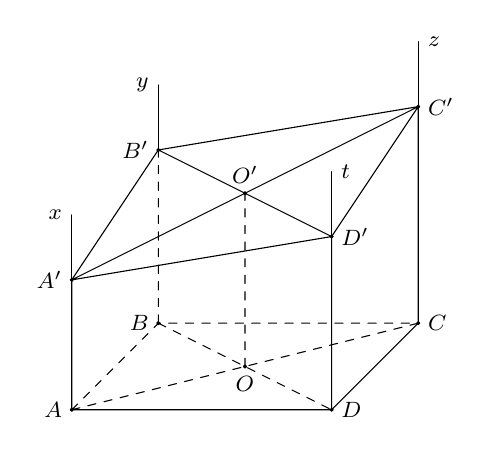
\begin{tikzpicture}[scale=0.55, font=\footnotesize, line join=round, line cap=round, >=stealth]
			\coordinate (A) at (0,0);	
			\coordinate (B) at (2,2);
			\coordinate	(C) at (8,2);	
			\coordinate	(D) at (6,0);
			\coordinate (M) at (0,3);	
			\coordinate (N) at (2,6);
			\coordinate	(P) at (8,7);	
			\coordinate	(Q) at (6,4);
			\coordinate	(I) at (4,1); 	
			\coordinate	(J) at (4,5);
			\coordinate	(U) at (0,4.5);
			\coordinate	(V) at (2,7.5);
			\coordinate	(S) at (8,8.5);
			\coordinate	(T) at (6,5.5);
			\draw (M)--(N)--(P)--(Q)--(M) (A)--(M) (Q)--(D) (P)--(C) (M)--(P) (N)--(Q) (A)--(D)--(C);
			\draw[dashed] (A)--(B)--(C) (B)--(N) (A)--(C) (B)--(D) (I)--(J);
			\draw (M)--(U) (N)--(V) (P)--(S) (Q)--(T);
			\draw[fill=black] (A) node[left]{$A$} circle(1pt);
			\draw[fill=black] (B) node[left]{$B$} circle(1pt);
			\draw[fill=black] (C) node[right]{$C$} circle(1pt);
			\draw[fill=black] (D) node[right]{$D$} circle(1pt);
			\draw[fill=black] (M) node[left]{$A'$} circle(1pt);
			\draw[fill=black] (N) node[left]{$B'$} circle(1pt);
			\draw[fill=black] (P) node[right]{$C'$} circle(1pt);
			\draw[fill=black] (Q) node[right]{$D'$} circle(1pt);
			\draw[fill=black] (U) node[left]{$x$};
			\draw[fill=black] (V) node[left]{$y$};
			\draw[fill=black] (S) node[right]{$z$};
			\draw[fill=black] (T) node[right]{$t$};
			\draw[fill=black] (I) node[below]{$O$} circle(1pt);
			\draw[fill=black] (J) node[above]{$O'$} circle(1pt);
			%	\draw[fill=black] (S) node[above]{$S$} circle(1pt);
			%	\draw[fill=black] (M) node[above left]{$M$} circle(1pt);
			%	\draw[fill=black] (N) node[above right]{$N$} circle(1pt);
		\end{tikzpicture}
	}
	\loigiai{
		\begin{enumerate}
			\item Ta có $AB\parallel CD$, $AA'\parallel DD'$, suy ra mp$(AA',BB')$ song song với mp$(CC',DD')$.
			\item Mặt phẳng $(P')$ cắt hai mặt phẳng song song mp$(AA',BB')$ và mp$(CC',DD')$ theo giao tuyến $A'B'$ và $C'D'$ suy ra $A'B'\parallel C'D'$.\\
			Tương tự ta cũng có $A'D'\parallel B'C'$.\\
			Tứ giác $A'B'C'D'$ có các cặp cạnh đối song song nên là hình bình hành.
			\item Do hai mặt phẳng $(AA'C'C)$ và $(BB'D'D)$ lần lượt chứa hai đường song song $AA'$ và $DD'$, cắt nhau theo giao tuyến $OO'$, nên $OO' \parallel AA'$.
		\end{enumerate}
	}
\end{vd}
\begin{vd}%[1H4H4-2]%[Dự án đề cương 3 khối NH24-25-Dot2-Huỳnh Đức Vũ]
	Cho hình chóp $S.ABCD$ có đáy $ABCD$ là hình bình hành và $O$ là giao điểm của hai đường chéo. Mặt phẳng $(P)$ đi qua điểm $O$ và song song với mặt phẳng $(SBC)$. Xác định giao tuyến của mặt phẳng $(P)$ với các mặt phẳng $(A B C D)$ và $(SCD)$.
	\loigiai{
		\immini{Do $(P) \parallel(S B C)$, $(A B C D) \cap(S B C)=B C$, $O$ là điểm chung của hai mặt phẳng $(P)$ và $(A B C D)$ nên giao tuyến $d$ của $(P)$ và $(A B C D)$ là đường thẳng đi qua $O$ và song song với $B C$.
			Gọi $N$ là giao điểm của $d$ và $C D$. Do $(S C D) \cap(S B C)=S C$, $(P) \parallel(S B C)$, $N$ là điểm chung của hai mặt phẳng $(P)$ và $(S C D)$ nên giao tuyến $d'$ của $(P)$ và $(S C D)$ là đường thẳng đi qua $N$ và song song với $S C$.}{\begin{tikzpicture}[scale=0.9, font=\footnotesize, line join=round, line cap=round, >=stealth]
				\path 
				(0,0) coordinate (D)
				($(D)+(-135:3)$) coordinate (A)
				($(A)+(0:5)$) coordinate (B)
				($(B)+(D)-(A)$) coordinate (C)
				($(D)!0.5!(B)$) coordinate (O)
				($(D)!0.5!(A)$) coordinate (I)
				($(D)!0.5!(C)$) coordinate (N)
				($(A)!0.5!(B)$) coordinate (K)
				($(I)+(90:5)$) coordinate (S)
				($(S)!0.5!(D)$) coordinate (H);
				\draw [dashed] (A)--(D)--(C) (S)--(D)--(B) (A)--(C) (N)--(K);
				\draw [dashed] (N)--(H) node[midway,above]{$d'$};
				\draw ($(O)+(0.2,0.3)$) node [above] {$d$};
				\draw (S)--(B) (S)--(A) (A)--(B)--(C)--(S) ;
				\foreach \x/\g in {A/180,D/180,C/0,B/0,O/-90,S/90,N/45}
				\fill[black] (\x) circle (1pt) + (\g:3mm) node {$\x$};
		\end{tikzpicture}}
	}
	
\end{vd}
\begin{vd}%[1H4H4-2]%[Dự án đề cương 3 khối NH24-25-Dot2-Huỳnh Đức Vũ]
Cho hình chóp $S.ABC$, lấy điểm $O$ thuộc miền trong tam giác $ABC$, điểm $I$ thuộc đoạn $SO$. Gọi $(\alpha)$ là mặt phẳng qua $I$ và song song với $(SBC)$. Tìm giao tuyến của 
	\begin{enumerate}
		\item Mặt phẳng $(IEF)$ và mặt phẳng $(ABC)$.
		\item Mặt phẳng $(IEF)$ và mặt phẳng $(SAC)$.
	\end{enumerate}
	\loigiai{
		\begin{center}
			\begin{tikzpicture}[scale=0.7,line cap=round,line join =round]
				\coordinate (A) at(0,0);
				\coordinate (B) at(3,-4);
				\coordinate (C) at(10,0);
				\coordinate (S) at($(A)+(0,7)$);
				\coordinate (O) at($(A)+(3.5,-1)$);
				\coordinate (I) at($(S)!0.7!(O)$);
				\coordinate (M) at (intersection cs:first line={(A)--(O)}, second line={(C)--(B)});
				\coordinate (x) at($(I)+(S)-(M)$);
				\coordinate(G) at (intersection cs:first line={(I)--(x)}, second line={(S)--(A)});
				\coordinate(J) at (intersection cs:first line={(I)--(G)}, second line={(M)--(A)});
				\coordinate (y) at($(J)+(B)-(M)$);
				\coordinate (E) at (intersection cs:first line={(J)--(y)}, second line={(B)--(A)});
				\coordinate (F) at (intersection cs:first line={(J)--(y)}, second line={(C)--(A)});
				
				\draw[dashed](A)--(C) (S)--(O) (G)--(J) (G)--(F) (A)--(M) (E)--(F);
				\draw (S)--(A)--(B)--(C)--(S)--(B);
				\foreach \i/\g in {A/180,B/-90,C/-90,E/180,F/40,O/-90,J/-90,M/-90,G/180,S/90,I/90}
				\fill[black] (\i) circle(1pt) ($(\i)+(\g:3.5mm)$) node{$\i$};
			\end{tikzpicture}
		\end{center}
		\begin{enumerate}
			\item Tìm giao tuyến của mặt phẳng $(IEF)$ và mặt phẳng $(ABC)$.\\
			Gọi $MF=AO\cap BC$.\\
			Ta có\\
			$\heva{&(\alpha)\parallel (SBC)\\ & (SAM)\cap (SBC)=SM\\ &(\alpha)\cap (SAM)=I} \Leftrightarrow (\alpha)\cap (SAM)=Ix$ với $\heva{& Ix\cap SA=G\\& Ix\cap AM= J \\& Ix\parallel SM.}$\\
			Do đó,\\
			$\heva{&(\alpha)\parallel (SBC)\\ & (ABC)\cap (SBC)=SM\\ &(\alpha)\cap (ABC)=J} \Leftrightarrow (\alpha)\cap (ABC)=EF$, với $\heva{& EF \mbox{ qua } J\\ &E\in AB, F\in AC\\ & EF\parallel SM.}$\\
			\item Tìm giao tuyến của mặt phẳng $(IEF)$ và mặt phẳng $(SAC)$.\\
			Ta có\\
			$\heva{&(\alpha)\parallel (SBC)\\ & (SAB)\cap (SBC)=SB\\ &(\alpha)\cap (SAB)=E} \Leftrightarrow (\alpha)\cap (SAB)=EG$, với $\heva{& G\in SA\\& EG\parallel SB.}$
		\end{enumerate}
	}
\end{vd}
\begin{dang}{Ứng dụng định lý Thales trong không gian}
\immini{Nếu hai cát tuyến $d$ và $d'$ cắt lần lượt ba mặt phẳng đôi một song song $(P)$, $(Q)$, $(R)$ lần lượt tại các điểm $A$, $B$, $C$ và $A'$, $B'$, $C'$  thì $\dfrac{AB}{A'B'}=\dfrac{BC}{B'C'}=\dfrac{CA}{C'A'}$.}{\begin{tikzpicture}[>=stealth,line join=round,line cap=round,font=\footnotesize,scale=0.8]
		\path
		(4,0) coordinate (uq)
		(3.2,0) coordinate (up)
		(4.8,0) coordinate (ur)
		(1,1.4) coordinate (vq)
		(0.8,1.2) coordinate (vp)
		(1.2,1.5) coordinate (vr)
		(0,0) coordinate (q)
		(0.75,2) coordinate (p)
		(-0.75,-2) coordinate (r)
		($(q)+(uq)$) coordinate (q1)
		($(q)+(vq)$) coordinate (q2)
		($(q1)+(q2)-(q)$) coordinate (q3)
		($(p)+(up)$) coordinate (p1)
		($(p)+(vp)$) coordinate (p2)
		($(p1)+(p2)-(p)$) coordinate (p3)
		($(r)+(ur)$) coordinate (r1)
		($(r)+(vr)$) coordinate (r2)
		($(r1)+(r2)-(r)$) coordinate (r3)
		(2.5,4) coordinate (x)
		(1,-3) coordinate (x4)
		(3,4) coordinate (y)
		(4,-3) coordinate (y4)
		(intersection of x--x4 and p--p1) coordinate (x1) 
		(intersection of x--x4 and q--q1) coordinate (x2) 
		(intersection of x--x4 and r--r1) coordinate (x3) 
		(intersection of y--y4 and p--p1) coordinate (y1) 
		(intersection of y--y4 and q--q1) coordinate (y2) 
		(intersection of y--y4 and r--r1) coordinate (y3) 
		($(x)!.7!(x1)$) coordinate (A)
		($(x)!.81!(x2)$) coordinate (B)
		($(x)!.8!(x3)$) coordinate (C)
		($(y)!.6!(y1)$) coordinate (A')
		($(y)!.85!(y2)$) coordinate (B')
		($(y)!.93!(y3)$) coordinate (C')
		;
		\draw 
		(p)--(p1)--(p3)--(p2)--cycle
		(q)--(q1)--(q3)--(q2)--cycle
		(r)--(r1)--(r3)--(r2)--cycle
		(x)--(A) (x1)--(B) (x2)--(C) (x3)--(x4)
		(y)--(A') (y1)--(B') (y2)--(C') (y3)--(y4)
		(A)--(A') (B)--(B') (C)--(C')
		;
		\draw[dashed] 
		(A)--(x1) (B)--(x2) (C)--(x3)
		(A')--(y1) (B')--(y2) (C')--(y3)
		;
		\begin{scope}
			\clip (q1)--(q)--(q2);
			\draw (q) circle (.8cm);
			\draw ($(q)+(30:.5cm)$) node{$Q$};
		\end{scope}
		\begin{scope}
			\clip (p1)--(p)--(p2);
			\draw (p) circle (.8cm);
			\draw ($(p)+(30:.5cm)$) node{$P$};
		\end{scope}
		\begin{scope}
			\clip (r1)--(r)--(r2);
			\draw (r) circle (.8cm);
			\draw ($(r)+(30:.5cm)$) node{$R$};
		\end{scope}
		\foreach \p/\g in {A/180, B/180, C/180, A'/0, B'/0, C'/0}
		\draw[fill=black] (\p) circle (1pt) node[shift=(\g:3mm)] {$\p$};
		\draw (x) node[below left] {$d$};
		\draw (y) node[below right] {$d'$};
\end{tikzpicture}}
	\end{dang}
\setcounter{vd}{0}
\begin{vd}%[1H4H4-2]%[Dự án đề cương 3 khối NH24-25-Dot2-Huỳnh Đức Vũ]
	Cho hình tứ diện $SABC$. Trên cạnh $SA$ lấy các điểm $A_1$, $A_2$ sao cho $AA_1=2A_1A_2=2A_2S$. Gọi $(P)$, $(Q)$ là hai mặt phẳng song song với mặt phẳng $(ABC)$ và lần lượt đi qua $A_1$, $A_2$. Mặt phẳng $(P)$ cắt các cạnh $SB$, $SC$ lần lượt tại $B_1$, $C_1$. Mặt phẳng $(Q)$ cắt các cạnh $SB$, $SC$ lần lượt tại $B_2$, $C_2$. Chứng minh $BB_1=2B_1B_2=2B_2S$ và $CC_1=2C_1C_2=2C_2S$.
	\loigiai
	{
		\immini
		{
			Áp dụng định lí Thalès cho ba mặt phẳng đôi một song song $(P)$, $(Q)$, $(ABC)$ và hai cát tuyến $SA$, $SB$ ta có $$\dfrac{B_2B_1}{B_1B}=\dfrac{A_2A_1}{A_1A}=\dfrac{1}{2}\Rightarrow BB_1=2B_1B_2.$$
	Vì $(P) \parallel (Q)$, $(SAB)\cap (P)=A_1B_1$, $(SAB)\cap (Q)=A_2B_2$ nên	$A_1B_1 \parallel A_2B_2$. Kết hợp với $A_1A_2=A_2S$, ta có $B_1B_2=B_2S$.\\
	Tương tự với hai cát tuyến $SA$, $SC$ suy ra $CC_1=2C_1C_2$ và $B_2C_2 \parallel B_1C_1$ nên $C_1C_2=C_2S$.
		}
		{
			\begin{tikzpicture}[>=stealth,line join=round,line cap=round,font=\footnotesize,scale=.65]
				\path 
				(0,0) coordinate (A)
				(3,-1.5) coordinate (B)
				(5.5,0) coordinate (C)
				(2,4.5) coordinate (S)
				($(A)!1/2!(S)$) coordinate (a1)
				($(S)!1/2!(a1)$) coordinate (a2)
				($(B)!1/2!(S)$) coordinate (b1)
				($(S)!1/2!(b1)$) coordinate (b2)
				($(C)!1/2!(S)$) coordinate (c1)
				($(S)!1/2!(c1)$) coordinate (c2)
				;
				\begin{scope}
					\fill[black!20]
					(a1)--(b1)--(c1)--cycle
					(a2)--(b2)--(c2)--cycle
					;
				\end{scope}
				\draw 
				(S)--(A)--(B)--(C)--(S)--(B)
				(a1)--(b1)--(c1)
				(a2)--(b2)--(c2)
				;
				\draw[dashed]
				(A)--(C) (a1)--(c1) (a2)--(c2)
				;
				\draw[fill=black]
				(A) circle (1pt) node[left] {$A$}
				(B) circle (1pt) node[below] {$B$}
				(C) circle (1pt) node[right] {$C$}
				(S) circle (1pt) node[above] {$S$}
				(a1) circle (1pt) node[shift=(135:3mm)] {$A_1$}
				(b1) circle (1pt) node[shift=(-30:3mm)] {$B_1$}
				(c1) circle (1pt) node[shift=(15:3mm)] {$C_1$}
				(a2) circle (1pt) node[shift=(135:3mm)] {$A_2$}
				(b2) circle (1pt) node[shift=(-30:3mm)] {$B_2$}
				(c2) circle (1pt) node[shift=(15:3mm)] {$C_2$}
				;
			\end{tikzpicture}
		}
	}
\end{vd}
\begin{vd}%[1H4H4-2]%[Dự án đề cương 3 khối NH24-25-Dot2-Huỳnh Đức Vũ]
	Cho hai hình bình hành $A B C D$ và $A B E F$ không cùng nằm trong một mặt phẳng.
	\begin{enumerate}[a)]
		\item Chứng minh rằng $(A F D) \parallel(B E C)$.
		\item  Gọi $M$ là trọng tâm của tam giác $A B E$. Gọi $(P)$ là mặt phẳng đi qua $M$ và song song với mặt phẳng $(A F D)$. Mặt phẳng $(P)$ cắt đường thẳng $A C$ tại $N$. Tính $\dfrac{A N}{N C}$.
	\end{enumerate}
	\loigiai{
		\begin{center}
			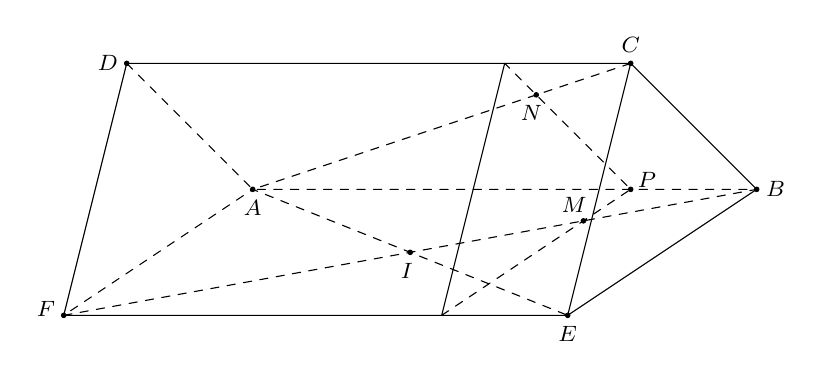
\begin{tikzpicture}[scale=0.8, font=\footnotesize, line join=round, line cap=round, >=stealth]
				\path 
				(0,0) coordinate (A)
				(8,0) coordinate (B)
				(6,2) coordinate (C)
				(-2,2) coordinate (D)
				(5,-2) coordinate (E)
				(-3,-2) coordinate (F)
				(6,0) coordinate (P)
				(4,2) coordinate (Q)
				(3,-2) coordinate (R)
				(intersection of A--E and B--F) coordinate (I)
				(intersection of A--C and P--Q) coordinate (N)
				(intersection of P--R and B--F) coordinate (M);
				\draw (D)--(C)--(B)--(E)--(F)--(D)--cycle(R)--(Q) (E)--(C) ;
				\draw[dashed] (D)--(A)--(B)--(F)--(A)--(E) (R)--(P)--(Q) (C)--(A);
				\foreach \i/\j in {A/270, B/0, C/90, D/180, E/270, F/160, P/30, I/-100, M/120, N/-105} \draw[fill=black] (\i) circle (1pt) ++(\j:0.3) node {$\i$};
			\end{tikzpicture}
			\end{center}
		\begin{enumerate}[a)]
			\item Vì $A B C D$ là hình bình hành nên $A D \parallel B C$. \\
		Mà $A D$ không thuộc mặt phẳng $(B E C)$, suy ra $A D \parallel(B E C)$. Tương tự, do $A B E F$ là hình bình hành nên $A F \parallel B E$, suy ra $A F \parallel(B E C)$. Mà $A D$, $A F$ cắt nhau nên $(A F D) \parallel(B E C)$.
				\item  Gọi $I$ là giao điểm của $A E$ và $B F$.
				Ta có $I$ là trung điểm đoạn $A E$ và $M$ là trọng tâm của tam giác $A B E$ nên $M \in B I$ và $B M=\dfrac{2}{3} B I=\dfrac{1}{3} B F$, hay $F M=2 M B$.
				Vì $(A F D) \parallel(B E C)$, $(A F D) \parallel(P)$ nên $(P) \parallel(B E C)$.
				Ta có đường thẳng $F B$ cắt ba mặt phẳng song song $(A D F)$, $(P)$, $(B C E)$ lần lượt tại $F$, $M$, $B$; đường thẳng $A C$ cũng cắt ba mặt phẳng trên theo thứ tự tại $A$, $N$, $C$.
				Áp dụng định lí Thalès trong không gian, ta có $$\dfrac{A N}{F M}=\dfrac{N C}{M B} \Rightarrow \dfrac{A N}{N C}=\dfrac{F M}{M B}=2.$$
				Vậy $\dfrac{A N}{N C}=2$.			
	\end{enumerate}}	
\end{vd}
\begin{vd}%[1H4V4-2]%[Dự án đề cương 3 khối NH24-25-Dot2-Huỳnh Đức Vũ]
	\immini{Một kệ để đồ bằng gỗ có mâm tầng dưới $(ABCD)$ và mâm tầng trên $(EFGH)$ song song với nhau. Bác thợ mộc đo được $AE=80$ cm, $CG=100$ cm và muốn đóng thêm một mâm tầng giữa $(IJKL)$ song song với hai mâm tầng trên và dưới sao cho khoảng cách $EI=50$ cm (Hình bên). Hãy giúp bác thợ mộc tính độ dài $GK$ để đặt mâm tầng giữa cho kệ để đồ đúng vị trí.}{
			\begin{tikzpicture}[line join=round, line cap=round, >=stealth, font=\footnotesize, scale=0.5]
				% Định nghĩa các điểm
				\coordinate (A) at (0,0);
				\coordinate (B) at (1.5,1);
				\coordinate (D) at (5,0);
				\coordinate (C) at (6.5,1);				
				\coordinate (E) at (0,5);
				\coordinate (F) at (1.5,6);
				\coordinate (H) at (3.5,5);
				\coordinate (G) at (5,6);				
				% Các điểm chia tỉ lệ 0.4 trên cạnh bên
				\coordinate (I) at ($(E)!0.4!(A)$);
				\coordinate (J) at ($(F)!0.4!(B)$);
				\coordinate (L) at ($(H)!0.4!(D)$);
				\coordinate (K) at ($(G)!0.4!(C)$);
				% Vẽ các cạnh nhìn thấy
				\draw (A)--(D)--(C)--(G)--(F)--(E)--(A)--(E)--(H)--(D);
				\draw (G)--(C);
				\draw (H)--(G);
				\draw (F)--(G);
				\draw (I)--(L);
				\draw (L)--(K);
				% Vẽ các cạnh khuất (đường đứt)
				\draw[dashed] (A)--(B)--(C);
				\draw[dashed] (B)--(F);
				\draw[dashed] (I)--(J)--(K);
				
				% Tô các điểm và ghi nhãn
				\foreach \pt/\ang in {A/180, B/-70, C/0, D/-50, 
					I/190, J/150, K/30, L/-120, 
					E/180, F/90, G/60, H/120}
				\fill (\pt) circle (1pt) node[shift={(\ang:0.3)}] {$\pt$};				
			\end{tikzpicture}		
	}	
	\loigiai{
		Ta có cát tuyến $EA$ cắt ba mặt phẳng song song $(EFGH)$, $(IJKL)$, $(ABCD)$ lần lượt tại $E$, $I$, $A$; cát tuyến $GC$ cũng cắt ba mặt phẳng trên theo thứ tự tại $G$, $K$, $C$. \\Áp dụng định lí Thalès trong không gian, ta có $\dfrac{EI}{GK}=\dfrac{AE}{CG}=\dfrac{80}{100}=\dfrac{4}{5}$.\\ Suy ra $GK=\dfrac{5}{4} EI=\dfrac{5}{4} \cdot 50 = 62{,}5$ (cm).\\
		Vậy độ dài $GK=62{,}5$ cm.}
\end{vd}
\subsection{BÀI TẬP LUYỆN TẬP}
\subsubsection{Bài tập trắc nghiệm nhiều lựa chọn}
\Opensolutionfile{ans}[ans/ans-1H1BAI4-ABCD]
\begin{ex}%[1H4N4-1]%[Dự án đề cương 3 khối NH24-25-Dot2-Huỳnh Đức Vũ]
	Cho đường thẳng $a$ song song với mặt phẳng $(P)$. Có bao nhiêu mặt phẳng chứa $a$ và song song với $(P)$?
	\choice
	{$0$}
	{\True  $1$}
	{ $2$}
	{Vô số}
	\loigiai{Cho đường thẳng $a$ song song với mặt phẳng $(P)$. Khi đó, có bao duy nhất một mặt phẳng chứa $a$ và song song với $(P)$.}
\end{ex}

\begin{ex}%[1H4N4-1]%[Dự án đề cương 3 khối NH24-25-Dot2-Huỳnh Đức Vũ]
	Cho mặt phẳng $(P)$ song song với mặt phẳng $(Q)$. Khẳng định nào sau đây là đúng?
	\choice
	{Mọi đường thẳng nằm trong $(P)$ đều song song với mọi đường thẳng nằm trong $(Q)$}
	{\True  $(P)$ song song với mọi đường thẳng nằm trong $(Q)$}
	{ Nếu mặt phẳng $(R)$ song song với mặt phẳng $(P)$ thì mặt phẳng $(R)$ song song với mặt phẳng $(Q)$}
	{ Nếu đường thẳng $a$ song song với mặt phẳng $(Q)$ thì đường thẳng $a$ song song với mặt phẳng $(P)$}
	\loigiai{ Cho mặt phẳng $(P)$ song song với mặt phẳng $(Q)$. Khi đó, mọi đường thẳng nằm trong mặt phẳng này đều song song với mặt phẳng kia.}
\end{ex}
\begin{ex}%[1H4N4-1]%[Dự án đề cương 3 khối NH24-25-Dot2-Huỳnh Đức Vũ]
	Điều kiện cần và đủ để hai mặt phẳng song song với nhau là
	\choice
	{Có một mặt phẳng chứa hai đường thẳng phân biệt cùng song song với mặt phẳng còn lại}
	{\True Hai mặt phẳng đó không có điểm chung}
	{Hai mặt phẳng đó cùng song song với một mặt phẳng thứ ba}
	{Hai mặt phẳng đó cùng song song với một đường thẳng}
	\loigiai{
		Điều kiện cần và đủ để hai mặt phẳng song song với nhau là hai mặt phẳng đó không có điểm chung.
	}
\end{ex}
\begin{ex}%[1H4N4-1]%[Dự án đề cương 3 khối NH24-25-Dot2-Huỳnh Đức Vũ]
	Tìm mệnh đề \textbf{sai} trong các mệnh đề sau.
	\choice
	{Nếu một đường thẳng cắt một trong hai mặt phẳng song song với nhau thì sẽ cắt mặt phẳng còn lại}
	{Nếu hai mặt phẳng phân biệt cùng song song với mặt phẳng thứ ba thì song song với nhau}
	{\True Nếu hai đường thẳng phân biệt cùng song song với một mặt phẳng thì song song với nhau}
	{Nếu hai mặt phẳng có một điểm chung thì chúng còn vô số điểm chung khác nữa}
	\loigiai{
		\immini{
			Xét hình hộp (thực tế có thể tận dụng căn phòng hình hộp chữ nhật hoặc hộp giấy hình hộp chữ nhật) là phản ví dụ cho phương án sai.
			Hai đường thẳng phân biệt $D'C'$ và $CC'$ cùng song song với mặt phẳng $(ABB'A')$ nhưng chúng cắt nhau tại $C'$.
		}{
			\begin{tikzpicture}[line join=round,line width=.7pt,font=\footnotesize,scale=.5]
				\def\a{3.5}\def\b{2.5}\def\h{3.5}\def\g{30}
				\path (0,\h) coordinate (A)--++(\g:\b) coordinate (B)--++(0:1.4*\a) coordinate (C)--++(\g-180:\b) coordinate (D)
				\foreach \x in {A,B,C,D}{($(\x)+(70:\h)$) coordinate (\x')};
				%\fill[opacity=.6,green!50] (A)--(B)--(B')--(A')--cycle;
				\draw[dashed] (B)--(B') (A)--(B)--(C);
				\draw (C)--(C')--(D')--(A')--(B')--(C') (C)--(D)--(A)--(A') (D)--(D');
				\foreach \p/\g in {A/-150,B/-70,C/-30,D/-70,A'/150,B'/90,C'/30,D'/-30}\draw[fill=black] (\p) circle (1pt)node[shift={(\g:.3)}]{$\p$};
			\end{tikzpicture}
		}
	}
\end{ex}

\begin{ex}%[1H4H4-2]%[Dự án đề cương 3 khối NH24-25-Dot2-Huỳnh Đức Vũ]
	\immini
	{Cho hình lăng trụ $ABC.A'B'C'$. Gọi $M$, $N$, $P$ theo thứ tự là trung điểm của các cạnh $AA'$, $BB'$, $CC'$.Mặt phẳng $(MNP)$ song song với mặt phẳng nào trong các mặt phẳng sau đây?
		\choice[2]
		{$(BMN)$}
		{$(BCA')$}
		{$(A'C'C)$}
		{\True $(ABC)$}
	}
	{\begin{tikzpicture}[scale=0.8, font=\footnotesize,line join=round, line cap=round, >=stealth]
			\def\h{3.2}
			\path (0,0) coordinate (A) (3.5,0) coordinate (C) (1.5,-1.2) coordinate (B);
			\foreach \i in {A,B,C} {\path (\i)+(0.5,\h) coordinate (\i');}
			\foreach \i/\j/\k in {A/A'/M, B/B'/N, C/C'/P} \path ($(\i)!1/2!(\j)$) coordinate(\k);
			\draw (A')--(A)--(B)--(C)--(C')--(B')--(A')--(C') (B)--(B') (M)--(N)--(P);
			\draw[dashed] (A)--(C) (M)--(P);
			\foreach \diem/\pos in {A/180, B/-90, C/0, C'/60, A'/120, B'/80, M/180, N/220, P/0} \fill (\diem) node[shift={(\pos:0.3)}] {$\diem$} circle(1pt);
	\end{tikzpicture}}
	\loigiai
	{Vì $ABC.A'B'C'$ là hình lăng trụ nên các mặt bên là các hình bình hành.\\
		Mà $M$, $N$, $P$ theo thứ tự là trung điểm của $AA'$, $BB'$, $CC'$ nên $MN$, $MP$ lần lượt là đường trung bình của các hình bình hành $ABB'A'$, $ACC'A'$.\\
		Ta có $MN\not\subset (ABC)$, $MN\parallel AB$, $AB\subset (ABC)$ nên $MN\parallel (ABC)$.\\
		Tương tự, $MP\parallel (ABC)$.\\
		Mà $MN$, $MP$ là hai đường thẳng cùng nằm trong mặt phẳng $(MNP)$ và cắt nhau tại $M$, suy ra $(MNP)\parallel (ABC)$.}
\end{ex}

\begin{ex}[Trích đề kiểm tra cuối kì 1-THPT Tân Bình - Tp.HCM-Năm học 2024-2025]
%[1H4N4-2]%[Dự án đề cương 3 khối NH24-25-Dot2-Huỳnh Đức Vũ]
	\immini{Cho tứ diện $ABCD$, Gọi $M$, $N$, $P$ lần lượt là trung điểm của các cạnh $AB$, $BC$, $BD$. Mặt phẳng $(MNP)$ song song với mặt phẳng nào trong các mặt phẳng sau đây?
		\choice
		{$(ABC)$}
		{$(BCD)$}
		{\True $(ACD)$}
		{$(ABD)$}
	}{\begin{tikzpicture}[line join=round,line cap=round,font=\footnotesize,scale=.9]
			\coordinate[label=left:$D$] (D) at (0,0);
			\coordinate[label=below left:$B$] (B) at (1,-1);
			\coordinate[label=right:$C$] (C) at (4,0);
			\coordinate[label=above left:$A$] (A) at (1.2,3);
			\coordinate[label=above right:$M$] (M) at ($(A)!.5!(B)$);
			\coordinate[label=below:$N$] (N) at ($(C)!.5!(B)$);
			\coordinate[label=below left:$P$] (P) at ($(D)!.5!(B)$);
			\draw (D)--(B)--(C)--(A)--cycle (A)--(B);
			\draw (P)--(M)--(N);
			\draw[dashed] (D)--(C) (N)--(P);
			\fill (A)circle(1pt) (B)circle(1pt) (C)circle(1pt) (D)circle(1pt) (M)circle(1pt) (N)circle(1pt) (P)circle(1pt);
		\end{tikzpicture}
	}
	\loigiai{
		Ta có $\heva{&MN\parallel AC\\&MP\parallel AD}$ nên $(MNP)\parallel (ACD)$.
	}
\end{ex}
\begin{ex}%[1H4N4-2]%[Dự án đề cương 3 khối NH24-25-Dot2-Huỳnh Đức Vũ]
	Cho lăng trụ tam giác $ABC.A'B'C'$. Khẳng định nào sau đây đúng?
	\choice
	{$(A'BC') \parallel (AB'C)$}
	{$(ABC') \parallel (A'B'C)$}
	{$(A'BC) \parallel (AB'C')$}
	{\True $(ABC) \parallel (A'B'C')$}
	\loigiai
	{
		\immini
		{
			Theo tính chất của hình lăng trụ, ta có khẳng định đúng là $(ABC) \parallel (A'B'C')$.
		}
		{
			\begin{tikzpicture}[>=stealth,line join=round,line cap=round,font=\footnotesize,scale=.41]
				\path
				(0,0) coordinate (A)
				(2,-2) coordinate (B)
				(7,0) coordinate (C)
				(1,4) coordinate (n)
				($(A)+(n)$) coordinate (A')
				($(B)+(n)$) coordinate (B')
				($(C)+(n)$) coordinate (C')
				;
				\draw (A)--(B)--(C)--(C')--(A')--(B')--(C') (B')--(B) (A)--(A');
				\draw[dashed] (A)--(C);
				\foreach \p/\g in {A/180, B/-90, C/0, A'/180, B'/-45, C'/0}
				\draw[fill=black] (\p) circle (1pt) node[shift=(\g:3mm)] {$\p$};
			\end{tikzpicture}
		}
	}
\end{ex}

\begin{ex}%[1H4N4-2]%[Dự án đề cương 3 khối NH24-25-Dot2-Huỳnh Đức Vũ]
	Cho hình hộp $ABCD.A'B'C'D'$. Mặt phẳng $\left(BCC'\right)$ song song với mặt phẳng nào sau đây?
	\choice
	{$\left(CDA'\right)$}
	{$\left(A'C'A\right)$}
	{\True $\left(A'DD'\right)$}
	{$\left(DC'D'\right)$}
	\loigiai{
		\immini{Ta có $(BCB')$
			cũng là mp $(BCC'B')$, mà theo tính chất hình hộp thì $(BCC'B')\parallel (ADD'A')$.}{
			\begin{tikzpicture}[>=stealth,line join=round,line cap=round,font=\footnotesize,scale=1]
				\path
				(0,0)coordinate(A)
				(2.5,0)coordinate(B)
				(-60:1.7)coordinate(C)
				($(A)+(C)-(B)$)coordinate(D)
				($(A)+(0.5,2)$)coordinate(A')
				($(A')+(B)-(A)$)coordinate(B')
				($(A')+(C)-(A)$)coordinate(C')
				($(A')+(D)-(A)$)coordinate(D')
				;
				\draw[dashed](A')--(A)--(B) (A)--(D);
				\draw(A')--(D')--(D)--(C)--(B)--(B')--(C')--(D') (A')--(B') (C')--(C) ;
				\foreach \x/\g in {A/150,B/0,C/-90,D/-90,A'/90,B'/0,C'/-30,D'/180}\fill[black](\x)circle(1pt)+(\g:.3)node{$\x$};
			\end{tikzpicture}
		}
	}
\end{ex}
\begin{ex}%[1H4N4-2]%[Dự án đề cương 3 khối NH24-25-Dot2-Huỳnh Đức Vũ]
	Cho lăng trụ $ABC.A'B'C'$. Gọi $M,N$ lần lượt là trung điểm của $BC$ và $B'C'$. Mệnh đề nào sau đây là đúng?
	\choice
	{\True $(A'BN)\parallel (AC'M) $}
	{$B'M \parallel (AA'C') $}
	{$(A'MN)\parallel(ACC') $}
	{$CN\parallel (ABB') $}
	\loigiai{
		\immini{
			Vì $M,N$ lần lượt là trung điểm của $BC$ và $B'C'$ nên $MN\parallel BB', MN=BB'$.\\
			Mà $BB'\parallel AA', BB'=AA'$ nên $MN\parallel AA',MN=AA'$.\\
			Do đó $A'NMA$ là hình bình hành, nên $A'N\parallel AM$.\\
			Mặt khác, ta cũng có $BN\parallel MC'$ ($NC'MB$ là hình bình hành).\\
			Nhận thấy, $\heva{&A'N\parallel AM\\&BN\parallel C'M\\&A'N,BN\subset (A'NB)\\&AM,MC'\subset (AMC')}\Rightarrow (A'BN)\parallel (AC'M)$.
		}
		{\begin{tikzpicture}[scale=1,>=stealth, font=\footnotesize, line join=round, line cap=round]
				
				% Định nghĩa điểm
				\coordinate (A) at (0,0);
				\coordinate (B) at (1.2,-1.5);
				\coordinate (C) at (3.5,0);
				
				% Trung điểm H của AB
				\coordinate (H) at ($(A)!0.5!(B)$);
				
				% Tạo điểm A' bằng cách nâng H lên cao 4 đơn vị
				\coordinate (A') at ($(H)+(0,4)$);
				
				% Vector từ A đến A'
				\coordinate (vecAA') at ($(A') - (A)$);
				
				% Tịnh tiến B và C để tạo B', C'
				\coordinate (B') at ($(B)+(vecAA')$);
				\coordinate (C') at ($(C)+(vecAA')$);
				
				% Trung điểm M của BC
				\coordinate (M) at ($(B)!0.5!(C)$);
				
				% Trung điểm N của B'C'
				\coordinate (N) at ($(B')!0.5!(C')$);
				
				% Vẽ lăng trụ
				\draw[] (A) -- (B) -- (C) -- (C') -- (B') -- (A') -- cycle
				(A') -- (C')
				(B') -- (B)
				(A') -- (B)
				(A') -- (N)
				(B) -- (N)
				(M) -- (C') ;
				
				% Đoạn đứt nét (ẩn phía sau)
				\draw[dashed] (A) -- (M)(A) -- (C);
				
				% Chấm điểm
				\foreach \p in {A,B,C,A',B',C',M,N}
				\filldraw[black] (\p) circle (1pt);
				
				% Gắn nhãn
				\node[above left] at (A') {$A'$};
				\node[left] at (A) {$A$};
				\node[below] at (B) {$B$};
				\node[above] at (B') {$B'$};
				\node[right] at (C) {$C$};
				\node[right] at (C') {$C'$};
				\node[below] at (M) {$M$};
				\node[above] at (N) {$N$};				
			\end{tikzpicture}	}
	}
\end{ex}

\begin{ex}%[1H4N4-2]%[Dự án đề cương 3 khối NH24-25-Dot2-Huỳnh Đức Vũ]
	Cho hình chóp $S.ABCD$ có đáy $ABCD$ là hình bình hành tâm $O$. Gọi $M$, $N$ lần lượt là trung điểm các cạnh $SD$ và $CD$. Mặt phẳng $\left(OMN\right)$ song song với mặt phẳng nào sau đây?
	\choice
	{$\left(SAD\right)$}
	{$\left(SAC\right)$}
	{\True $\left(SBC\right)$}
	{$\left(SAB\right)$}
	\loigiai{
		\immini{
			Ta có $OM$, $MN$ là đường trung bình của tam giác $SBD$ và tam giác $SCD$ nên\\
			$\heva{&OM\parallel SB\\&MN\parallel SC} \Rightarrow \heva{&OM\parallel \left(SBC\right)\\&
				MN\parallel (SBC) } \Rightarrow\left(OMN\right)\parallel \left(SBC\right)$.}
		{\begin{tikzpicture}[scale=1, font=\footnotesize, line join=round, line cap=round, >=stealth]
				\path
				(0,0) coordinate (A)
				(-1.5,-1.5) coordinate (B)
				(4,0) coordinate (D)
				($(B)+(D)-(A)$) coordinate (C)
				(0,3) coordinate (S)
				($(S)!0.5!(D)$) coordinate (M)
				($(C)!0.5!(D)$) coordinate (N)
				($(A)!0.5!(C)$) coordinate (O)
				;
				\draw
				(S)--(B)--(C)--(D)--(S)--(C) (M)--(N)
				;
				\draw[dashed]
				(S)--(A)--(C)
				(B)--(A)--(D)--cycle
				(M)--(O)--(N)
				;
				\foreach \p/\g in {A/170, B/-90, C/-90, D/0, S/90, O/-90, M/80, N/-10}
				\draw[fill=black] (\p) circle (1pt) node[shift=(\g:3mm)] {$\p$};
				%\pic[draw,angle radius=2mm]{angle=A--H--O};
	\end{tikzpicture}}}
\end{ex}

\begin{ex}[Trích đề kiểm tra Toán 11 CHKI-THPT Trần Phú - Đà nẵng-năm học 2024-2025]
		%[1H4H4-2]%[Dự án đề cương 3 khối NH24-25-Dot2-Huỳnh Đức Vũ]
	\immini{Cho hình chóp tứ giác $S.ABCD$. Gọi $M$, $N$, $P$ lần lượt là trung điểm các cạnh $SA$, $AB$ và $AD$ \textit{(tham khảo hình vẽ)}. Mặt phẳng $(MNP)$ song song với mặt phẳng nào dưới đây?
		\choice
		{$(ABCD)$}
		{\True $(SBD)$}
		{$(SBC)$}
		{$(SCD)$}
	}
	{\begin{tikzpicture}[scale=0.8, font=\footnotesize,line join=round, line cap=round, >=stealth]
			\coordinate (A) at (0,0);
			\coordinate (B) at (1.2,-1.8);
			\coordinate (D) at (5,0);
			\coordinate (C) at (4,-2.0);
			\coordinate (S) at ($(A)+(2,3)$);
			\coordinate (M) at ($(S)!0.5!(A)$);
			\coordinate (N) at ($(B)!0.5!(A)$);
			\coordinate (P) at ($(D)!0.5!(A)$);
			\foreach \i in {A,B,C,D}{\draw (S)--(\i);}
			\draw (A)--(B)--(C)--(D) (M)--(N);
			\draw[dashed,thin] (A)--(D) (M)--(P)--(N);
			\foreach \i/\g in {S/90,A/180,B/-90,C/-90,D/0,M/135,N/-135,P/45}{\draw[fill=black](\i) circle (1pt) ($(\i)+(\g:3mm)$) node[scale=1]{$\i$};}
	\end{tikzpicture}}
	\loigiai{
		\immini{Ta có $\heva{&MN\parallel SB \\&NP\parallel BD\\&MN,NP\subset (MNP)\\& SB,BD \subset (SBD)}\Rightarrow (MNP) \parallel (SBD)$.}
		{\begin{tikzpicture}[scale=0.8, font=\footnotesize,line join=round, line cap=round, >=stealth]
				\coordinate (A) at (0,0);
				\coordinate (B) at (1.2,-1.8);
				\coordinate (D) at (5,0);
				\coordinate (C) at (4,-2.0);
				\coordinate (S) at ($(A)+(2,3)$);
				\coordinate (M) at ($(S)!0.5!(A)$);
				\coordinate (N) at ($(B)!0.5!(A)$);
				\coordinate (P) at ($(D)!0.5!(A)$);
				\foreach \i in {A,B,C,D}{\draw (S)--(\i);}
				\draw (A)--(B)--(C)--(D) (M)--(N);
				\draw[dashed,thin] (A)--(D) (M)--(P)--(N) (B)--(D);
				\foreach \i/\g in {S/90,A/180,B/-90,C/-90,D/0,M/135,N/-135,P/45}{\draw[fill=black](\i) circle (1pt) ($(\i)+(\g:3mm)$) node[scale=1]{$\i$};}
		\end{tikzpicture}}
	}
\end{ex}

\begin{ex}%[1H4H4-2]%[Dự án đề cương 3 khối NH24-25-Dot2-Huỳnh Đức Vũ]
	Cho tứ diện $ABCD$. Gọi $I$, $J$ lần lượt là trung điểm của $AB$, $BC$. Tìm mệnh đề đúng trong các mệnh đề sau.
	\choice
	{Giao tuyến của $(IJD)$ và $(BCD)$ là đường thẳng qua $C$ song song với $JD$}
	{\True Giao tuyến của $(IJD)$ và $(ACD)$ là đường thẳng qua $D$ song song với $IJ$}
	{Giao tuyến của $(IJD)$ và $(ABD)$ là đường thẳng qua $B$ song song với $ID$}
	{Giao tuyến của $(IJD)$ và $(ABD)$ là đường thẳng qua $A$ song song với $ID$}
	\loigiai{
		\immini
		{
			Xét hai mặt phẳng $(DIJ)$ và $(ACD)$, ta có
			\[\heva{&D\in(DIJ)\cap(ACD)\\&IJ\subset(DIJ)\\&AC\subset(ACD)\\&AC\parallel IJ}\Rightarrow(DIJ)\cap(ACD)=Dx\parallel AC\parallel IJ.\]
		}{
			\begin{tikzpicture}[>=stealth, line join=round, line cap = round, scale = 0.8, font=\footnotesize]
				
				% Định nghĩa các điểm
				\coordinate (B) at (0,0);
				\coordinate (D) at (6,0);
				\coordinate (C) at (2,-2);
				\coordinate (A) at (3,4);
				% Trung điểm I của AB
				\coordinate (I) at ($(A)!0.5!(B)$);
				% Trung điểm J của BC
				\coordinate (J) at ($(B)!0.5!(C)$);
				% Các điểm chính
				\foreach \p in {A,B,C,D,I,J}
				\filldraw[black] (\p) circle (1pt);
				% Các cạnh chính
				\draw (A) -- (B) -- (C) -- (D) -- (A) -- (C);
				\draw (I) -- (J);
				% Các cạnh khuất (dashed)
				\draw[dashed] (B) -- (D);
				\draw[dashed] (D) -- (I);
				\draw[dashed] (D) -- (J);
				% Nhãn điểm
				\node[left] at (B) {$B$};
				\node[below] at (C) {$C$};
				\node[right] at (D) {$D$};
				\node[above] at (A) {$A$};
				\node[above] at (I) {$I$};
				\node[below left] at (J) {$J$};
					% Trục x
				\draw (5.75,-1.5) -- (6.75,4.54) node[above]{$x$};
					\end{tikzpicture}
	
		
		
		
		}
	}
\end{ex}
\begin{ex}%[1H4H4-4]%[Dự án đề cương 3 khối NH24-25-Dot2-Huỳnh Đức Vũ]
	Cho hình chóp $S.ABCD$ có đáy $ABCD$ là hình thang $(AD \parallel BC$, $AD > BC)$. Gọi $M$ là điểm di động trên đoạn $AB$, $M$ không trùng với $A$. Qua $M$ vẽ mặt phẳng $(\alpha)$ song song với $(SBC)$. Gọi $d$ là giao tuyến của $(\alpha)$ và mặt phẳng $(SAD)$. Kết luận nào sau đây đúng về $d$?
	\choice
	{$ d$ cắt $(ABCD)$}
	{$d$ cắt $AD$}
	{\True $d \parallel AD$}
	{$ d$ cắt $BC$}
	\loigiai{
		\immini{Vì $(\alpha ) \parallel ( SBC )$ nên $(\alpha ) \parallel BC$, $(\alpha ) \parallel SC$.\\
			Vì $M$ khác $A$ nên $AD\not \subset (\alpha)$. Từ $AD\parallel BC$ và $BC\parallel (\alpha)$, ta có $(\alpha \parallel AD)$.
			Vì $(\alpha ) \parallel BC$ và $(\alpha)$ đi qua điểm $M \in (ABCD)$ nên $(\alpha)$ cắt $(ABCD)$ theo một giao tuyến $d_1$ qua $M$ và $d_1\parallel BC$. Gọi $N=d_1\cap CD$.\\
			Vì $(\alpha ) \parallel SC$ và $(\alpha)$ đi qua điểm $N \in (SCD)$ nên $(\alpha)$ cắt $(SCD)$ theo một giao tuyến $d_2$ qua $N$ và $d_2\parallel SC$. Gọi $P=d_2\cap SD$.\\	
			Vì $(\alpha ) \parallel AD$ và $(\alpha)$ đi qua điểm $P \in (SAD)$ nên $(\alpha)$ cắt $(SAD)$ theo một giao tuyến $d$ qua $P$ và $d\parallel AD$. 
		}{\begin{tikzpicture}[scale=0.8]
				\def\a{5}
				\def\h{4}
				\path   (0:0) coordinate (A)
				++(0:\a) coordinate (D)
				($(A)+(-130:\a/2)$) coordinate (B)
				($(D)+(B)-(A)$) coordinate (Ct)
				($(B)!1/2!(Ct)$) coordinate (C)
				($(A)+(90:\h)$) coordinate (S)
				($(A)!0.5!(B)$) coordinate (M)
				($(C)!0.5!(D)$) coordinate (N)
				($(S)!0.5!(D)$) coordinate (P)
				($(S)!0.5!(A)$) coordinate (Q)
				(intersection of A--C and D--B) coordinate (O);%giao điểm O
				\draw[dashed] (D)--(A)--(B)   (A)--(S) (N)--(M) (Q)--(P)node[pos=0.5,above]{$d$};
				\draw (D)--(C)--(B) (D)--(S) (C)--(S)    (B)--(S) (P)--(N);
				\foreach \x/\g in {A/135,D/45,C/-45,B/-135,S/90,M/-60,N/-30,P/45/}
				\fill[black]    (\x) circle (1pt)
				($(\g:3mm)+(\x)$) node {$\x$};
			\end{tikzpicture}
		}
	}
\end{ex}
\begin{ex}%[1H4H4-2]%[Dự án đề cương 3 khối NH24-25-Dot2-Huỳnh Đức Vũ]
	Cho hình chóp $S.ABCD$ có đáy là hình thang $(AB\parallel CD)$ và $AB=2CD$. Gọi $I$, $J$
	lần lượt là trung điểm của $SB$ và $AB$. Mặt phẳng nào song song với mặt phẳng $(SAD)$?
	\choice
	{$(BIJ)$}
	{$(SJC)$}
	{\True $(CIJ)$}
	{$(BCI)$}
	\loigiai{
		\begin{center}
			\begin{tikzpicture}[scale=1, font=\footnotesize, line join=round, line cap=round, >=stealth]
				\def\bc{4} % cạnh BC
				\def\ba{2} % cạnh BA
				\def\h{4} % đường cao
				\def\gocB{30} % góc B của đáy
				\path
				(0,0) coordinate (B)node[below]{$D$}
				(\gocB:\ba) coordinate (A)
				(\bc,0) coordinate (C)
				($(C)-(B)+(A)$) coordinate (J)
				($(J)!-1!(A)$) coordinate (D)node[right]{$B$}
				($(A)+(95:\h)$) coordinate (S)
				($(S)!.5!(D)$) coordinate (I)
				;
				\draw (B)--(C)--(D)--(S)--cycle (S)--(C)--(I)
				;
				\draw[dashed] (A)--(D) (S)--(A)--(B) (I)--(J)--(C);
				\foreach \x in {B,D}\fill[red] (\x) circle (1pt);
				\foreach \x/\g in {A/160,C/-45,S/90,J/-40,I/90}\fill (\x) circle (1pt)+(\g:3mm) node[black]{$ \x $};
			\end{tikzpicture}
		\end{center}
		Xét tam giác $SAB$, ta có $IJ\parallel SA\Rightarrow IJ\parallel(SAD)$. \qquad {$(1)$}\\
		Ta có tứ giác $ADCJ$ là hình bình hành suy ra $CJ\parallel AD\Rightarrow CJ\parallel(SAD)$. \qquad {$(2)$}\\
		Từ $(1)$, $(2)$ suy ra $(CIJ)\parallel(SAD)$.
	}
\end{ex}
\begin{ex}%[1H4H4-2]%[Dự án đề cương 3 khối NH24-25-Dot2-Huỳnh Đức Vũ]
	Cho hình lăng trụ $ABC.A'B'C'$. Gọi $I$, $J$, $K$ lần lượt là trọng tâm của tam giác $ABC$, $ACC'$, $A'B'C'$. Mặt phẳng nào sau đây song song với mặt phẳng $(IJK)$?
	\choice
	{$(ABC)$}
	{$(A'BC')$}
	{$(ABB')$}
	{\True $(BB'C')$}
	\loigiai{
		\immini{
			Gọi $M$ là trung điểm cạnh $AC$, ta có
			\begin{itemize}
				\item $I$ là trọng tâm $\triangle ABC$ nên $\dfrac{MI}{MB}=\dfrac{1}{3}$.
				\item $J$ là trọng tâm $\triangle ACC'$ nên $\dfrac{MJ}{MC'}=\dfrac{1}{3}$.
			\end{itemize}
			Do đó $\dfrac{MI}{MB}=\dfrac{MJ}{MC'}=\dfrac{1}{3}$, suy ra $IJ\parallel BC'$.\\
			Ta lại có $BIKB'$ là hình bình hành nên $IK\parallel BB'$.\\
			Khi đó $\heva{&IJ\parallel BC'\\&IK\parallel BB'}\Rightarrow (IJK)\parallel (BB'C')$.
		}
		{
			\begin{tikzpicture}[>=stealth,line join=round, line cap =round, font=\footnotesize, scale=.8]
				\def\goc{75}
				\path
				(0,0)coordinate(A)++(0:4)coordinate(B)++(230:2)coordinate(C)++(\goc:4)coordinate(C')
				(A)++(\goc:4)coordinate(A')
				(B)++(\goc:4)coordinate(B')
				($(A)!.5!(C)$)coordinate(M)
				($(B)!2/3!(M)$)coordinate(I)++(\goc:4)coordinate(K)
				($(C')!2/3!(M)$)coordinate(J)
				;
				\draw (K)--(B')--(B)--(C)--(A)--(A')--(B')--(C')--(C)
				(A')--(C')--(A) (B)--(C')--(M)
				;
				\draw[dashed] (A)--(B)--(M) (I)--(K)--(J)--cycle
				;
				\foreach \x/\g in {C/-90,A/180,B/0,B'/0,C'/90,A'/90,I/-90,K/90,J/150,M/-110}
				\fill[black] (\x)circle (1pt) ($(\x)+(\g:3mm)$)node{$\x$};
			\end{tikzpicture}
		}
	}
\end{ex}
\begin{ex}%[1H4H4-2]%[Dự án đề cương 3 khối NH24-25-Dot2-Huỳnh Đức Vũ]
	Cho hình hộp $ABCD.A'B'C'D'$. Mặt phẳng $(AB'D')$ song song với mặt phẳng
	\choice
	{\True $(BDC')$}
	{$(ABCD)$}
	{$(BDA')$}
	{$(BCC'B')$}
	\loigiai{
		\immini{Do $ABC'D'$ là hình bình hành nên $AB\parallel C'D'$.\\
			Do $ADC'B'$ là hình bình hành nên $AB'\parallel DC'$.\\
			Xét hai mặt phẳng $(AB'D')$ và $(C'BD)$ có\\
			$\heva{&AB'\parallel DC'\\& AB\parallel C'D'\\&AB''\,\text{và}\,AB\text{cắt nhau}}\Rightarrow (AB'D')\parallel(C'BD)$.}{\begin{tikzpicture}[scale=1,font=\footnotesize,line join = round, line cap = round, >= stealth]
				\coordinate (A) at (0,0);
				\def\x{4}
				\def\y{2}
				\def\z{2.5}
				\def\g{60}% goc hbh đáy
				\def\n{85} %goc nghiêng
				\coordinate (B) at ($(A)+(\x,0)$);
				\coordinate (D) at ($(A)+(\g:\y)$);
				\coordinate (C) at ($(B)+(D)-(A)$);
				\coordinate (A') at ($(A)+(\n:\z)$);
				\coordinate (B') at ($(B)+(\n:\z)$);
				\coordinate (C') at ($(C)+(\n:\z)$);
				\coordinate (D') at ($(D)+(\n:\z)$);
				\draw (A)--(B)--(B')--(A')--cycle;
				\draw (A')--(D')--(C')--(B');
				\draw (B)--(C)--(C');
				\draw (A)--(B')--(D') (B)--(C');
				\draw[dashed] (D')--(A)--(D)--(D') (C)--(D)--(C') (D)--(B);
				\foreach \p/\g in {A/180,B/-45,C/-45,D/-90,A'/90,B'/80,C'/90,D'/90} \draw (\p) circle(1pt) node [shift={(\g:.3)}] {$\p$};
		\end{tikzpicture}}
	}
\end{ex}
\begin{ex}%[1H4V4-2]%[Dự án đề cương 3 khối NH24-25-Dot2-Huỳnh Đức Vũ]
	\immini{Ông Hai có một kệ gỗ để vật dụng gia đình gồm 2 tầng song song nhau. Để tăng diện tích để vật dụng, ông Hai đóng thêm một mặt gỗ ở giữa hai tầng để trở thành kệ gỗ 3 tầng. Do đó, ông Hai kí hiệu và đo các kích thước như hình bên dưới. Nếu ông Hai đo đoạn $AM=20 \mathrm{~cm}$ thì ông Hai phải đo $CP$ dài bao nhiêu $\mathrm{cm}$ để mặt gỗ $MNPQ$ song song với 2 tầng kia? Biết $AE=60 \mathrm{~cm}, CG=66 \mathrm{~cm}$
		\choice
		{ $CP=30 \mathrm{~cm}$}
		{ $CP=25 \mathrm{~cm}$}
		{ $CP=20 \mathrm{~cm}$}
		{\True $CP=22 \mathrm{~cm}$}
	}{\begin{tikzpicture}[declare function={a=2;b=4;h=5;},line join=round,yscale=0.6]
			\path (0,0) coordinate (G)
			(35:a) coordinate (F)
			(b,0) coordinate (H)
			($(H)-(G)+(F)$) coordinate (E)
			($(F)+(90:h)$) coordinate (B)
			($(G)-(F)+(B)$) coordinate (C)
			($(H)-(F)+(B)$) coordinate (D)
			($(E)-(F)+(B)$) coordinate (A);
			\path ($(A)!0.2!(E)$) coordinate (M) ($(B)!0.2!(F)$) coordinate (N)
			($(C)!0.2!(G)$) coordinate (P) ($(D)!0.2!(H)$) coordinate (Q);
			\draw ( C)--(G)--(H)--(E)--(A)--(B)--(C)--(D)--(A)  (H)--(D) (P)--(Q)--(M);
			\draw[dashed]  (B)--(F)--(E)  (F)--(G) (P)--(N)--(M);
			\foreach \t/\g in {F/180,G/-90,H/-90,B/90,C/90,D/90,A/0,E/0,M/0,N/30,P/180,Q/-30}{
				\draw[fill=white] (\t) circle (1pt) node[shift={(\g:7pt)},font=\scriptsize]{$ \t $};
			}
	\end{tikzpicture}}
	\loigiai{
		Khi ba mặt phẳng song song thì áp dụng định Thalès trong không gian ta có
		\[
		\dfrac{CP}{CG}=\dfrac{AM}{AE} \Rightarrow CP = \dfrac{AM\cdot CG}{AE} = \dfrac{20\cdot 66}{60} = 22\mathrm{~cm}.
		\]
	}
\end{ex}
\begin{ex}[Trích đề kiểm tra Toán 11 CHKI-Chuyên Hùng Vương-Phú Thọ-Năm học 2024-2025]	%[1H4H4-3]%[Dự án đề cương 3 khối NH24-25-Dot2-Huỳnh Đức Vũ]
	\immini{Cho hình chóp $S.ABCD$ có đáy $ABCD$ là hình bình hành tâm $O$ (tham khảo hình vẽ). Gọi $M$, $N$ theo thứ tự là trung điểm $SA$, $SD$. Mặt phẳng $(OMN)$ song song với mặt phẳng nào sau đây?
		\choice
		{$(SAB)$}
		{\True $(SBC)$}
		{$(ABCD)$}
		{$(SCD)$}
	}
	{\begin{tikzpicture}[=>stealth,line join=round,line cap=round, font=\footnotesize, scale=.7]
			\def\a{4}
			\def\goc{210}
			\def\b{2.5}
			\def\h{4.5}
			\path
			(0,0)coordinate (A)++(0:\a)coordinate (D)++(\goc:\b)coordinate (C)++(180:\a)coordinate (B)
			(A)++(90:\h)coordinate (S)
			($(C)!1/2!(A)$)coordinate (O)
			($(S)!1/2!(A)$)coordinate (M)
			($(S)!1/2!(D)$)coordinate (N)
			;
			\draw (S)--(B)--(C)--(D)--cycle (S)--(C);
			\draw[dashed] (S)--(A)--(C) (B)--(A)--(D) (M)--(N)--(O)--(M) (B)--(D);
			\foreach \x/\g in{A/170,B/-90,C/-90,D/-90,S/90,O/-90,M/180,N/30}
			\fill[black](\x)circle(1pt) ($(\x)+(\g:3mm)$)node{$\x$}
			;
	\end{tikzpicture}}
	\loigiai{
		Vì $\heva{&MN \parallel AD \parallel BC\\&OM \parallel SC\\&MN,OM \subset (OMN)}$ nên $(OMN)\parallel (SBC)$.
	}
\end{ex}

\begin{ex}%[1H4V4-2]%[Dự án đề cương 3 khối NH24-25-Dot2-Huỳnh Đức Vũ]
	Cho hình lăng trụ $ABC.A'B'C'$. Gọi $I$, $J$, $K$ lần lượt là trọng tâm tam giác $ABC$, $ACC'$, $AB'C'$. Mặt phẳng nào sau đây song song với $(IJK)$?
	\choice
	{$(BC'A)$}
	{$(CC'A)$}
	{\True $(BB'C)$}
	{$(A'B'C')$}
	\loigiai{
		\immini{
			Do $I$, $J$, $K$ lần lượt là trọng tâm tam giác $ABC$, $ACC'$, $AB'C'$ nên ta có $$\dfrac{AI}{AM}=\dfrac{AJ}{AN}=\dfrac{2}{3}\Rightarrow IJ\parallel MN.$$
			Mà $IJ \not \subset (BCC'B')$ nên $ IJ\parallel (BCC'B')$.\qquad (1)\\
			Tương tự $IK\parallel (BCC'B')$.\qquad(2)\\
			Vì hai đường thẳng $IJ$ và $IK$ cắt nhau nên từ $(1)$ và $(2)$ ta có $(IJK)\parallel (BCC'B')$.
		}
		{
			\begin{tikzpicture}[scale=1, font=\footnotesize, line join=round, line cap=round, >=stealth]
				\def\a{4} \def\b{1.8} \def\h{4} \def\g{100}
				\path
				(0:0) coordinate (A)
				(0:\a) coordinate (C)
				(-60:\b) coordinate (B)
				($(A)+(\g:\h)$) coordinate (A')
				($(B)+(\g:\h)$) coordinate (B')
				($(C)+(\g:\h)$) coordinate (C')
				($(B)!1/2!(C)$) coordinate (M)
				($(C')!1/2!(C)$) coordinate (N)
				($(B')!1/2!(C')$) coordinate (P)
				($(A)!2/3!(M)$) coordinate (I)
				($(A)!2/3!(N)$) coordinate (J)
				($(A)!2/3!(P)$) coordinate (K)
				;
				\draw (B)--(B')--(C')--(A')--(B') (A')--(A)--(B)--(C)--(C')
				(M)--(N)--(P)--(M)
				;
				\draw[dashed]
				(A)--(C)
				(M)--(A)--(N)
				(A)--(P)
				(I)--(J)--(K)--(I)
				;
				\foreach \x/\g in {A/150,A'/150,B/180,B'/180,C/0,C'/0,M/-30,N/0,P/90,I/-90,J/45,K/120}
				\fill[black] (\x) circle(1pt) ($(\x)+(\g:3mm)$) node{$\x$};
			\end{tikzpicture}
		}
	}
\end{ex}

\begin{ex}[Trích đề kiểm tra cuối HKI-THPT Trần Quốc Toản-DakLak- Năm học NH2023-2024]
%[1H4V4-2]%[Dự án đề cương 3 khối NH24-25-Dot2-Huỳnh Đức Vũ]
	\immini{Cho hình chóp $S. ABCD$ đáy là hình thang, $AB \parallel CD$, $AB=a$; $CD=2 a$, gọi $I$ là giao điểm của $AC$ và $BD$. Qua $I$ kẻ đường thẳng song song $CD$ cắt $BC$ tại $M$. Trên cạnh $SC$ lấy điểm $N$ sao cho $CN=2NS$ (tham khảo hình bên)
		\choice
		{$(IMN) \parallel(SBD)$}
		{$(IMN) \parallel(SAC)$}
		{$(IMN) \parallel(SAD)$}
		{\True $(IMN) \parallel(SAB)$}
	}
	{\begin{tikzpicture}[=>stealth,line join=round,line cap=round, font=\footnotesize, scale=.7]
			\def\a{3}
			\def\goc{345}
			\def\b{5}
			\def\h{4}
			\path
			(0:0) coordinate (A)
			(A)++(80:\h)coordinate (S);
			\path
			(0,0)coordinate (A)++(0:\a)coordinate (B)++(\goc:\b)coordinate (C)++(180:2*\a)coordinate(D)
			($(C)!2/3!(S)$)coordinate (N)
			(A)++(80:\h)coordinate (S)
			($(C)!2/3!(B)$)coordinate (M)
			;
			\path (intersection of C--A and B--D)coordinate (I)%giao điểm 2 đt	
			;
			\draw (C)--(D)--(A)--(S) (D)--(S)--(C);
			\draw[dashed] (A)--(B)--(C)  (S)--(B)--(C) (A)--(C) (B)--(D) (I)--(M)
			;
			\foreach \x/\g in{A/180,B/40,C/-90,S/90,D/-90,I/-90,M/60,N/60}
			\fill[black](\x)circle(1pt) ($(\x)+(\g:3mm)$)node{$\x$}
			;
	\end{tikzpicture}}
	\loigiai{
		\immini{Ta có $\dfrac{MC}{MB}=\dfrac{NC}{NS}=2\Rightarrow MN\parallel SB$,\\
			và $IM \parallel DC \parallel AB$.\\
			Khi đó $\heva{&IM \parallel AB\\&MN\parallel SB\\&IM, MN \subset (IMN)\\&AB,SB \subset (SAB)}\Rightarrow (IMN) \parallel(SAB)$.
		}
		{\begin{tikzpicture}[=>stealth,line join=round,line cap=round, font=\footnotesize, scale=.7]
				\def\a{3}
				\def\goc{345}
				\def\b{5}
				\def\h{4}
				\path
				(0,0)coordinate (A)++(0:\a)coordinate (B)++(\goc:\b)coordinate (C)++(180:2*\a)coordinate(D)
				($(C)!2/3!(S)$)coordinate (N)
				(A)++(80:\h)coordinate (S)
				($(C)!2/3!(B)$)coordinate (M)
				;
				\path (intersection of C--A and B--D)coordinate (I)%giao điểm 2 đt	
				;
				\draw (C)--(D)--(A)--(S) (D)--(S)--(C);
				\draw[dashed] (A)--(B)--(C)  (S)--(B)--(C) (A)--(C) (B)--(D) (I)--(M)--(N)--(I);
				\foreach \x/\g in{A/180,B/40,C/-90,S/90,D/-90,I/-90,M/60,N/60}
				\fill[black](\x)circle(1pt) ($(\x)+(\g:3mm)$)node{$\x$}
				;
		\end{tikzpicture}}
	}
\end{ex}
\Closesolutionfile{ans}
%\indapan{10}{ans/ans-1H1BAI4-ABCD}
\subsubsection{Trắc nghiệm đúng sai}

\Opensolutionfile{ans}[ans/ans-1H1BAI4-DS]
\setcounter{ex}{0}
\begin{ex}[Trích Đề cuối kì 1-THPT Nguyễn Du-Bà Rịa Vũng Tàu-Năm học 2024-2025]
	%[1H4H4-2]%[Dự án đề cương 3 khối NH24-25-Dot2-Huỳnh Đức Vũ]
	Cho lăng trụ tứ giác $ABCD.A'B'C'D'$ có hai đáy $ABCD$ và $A'B'C'D'$ là hai hình bình hành.
	\choiceTF[t]
	{\True Mặt phẳng $(ACD')$ song song với mặt phẳng $(BA'C')$}
	{\True Lăng trụ tứ giác $ABCD.A'B'C'D'$ là một hình hộp}
	{Tứ giác $ABC'D'$ là hình chữ nhật}
	{\True Đường thẳng $AD'$ song song với mặt phẳng $(BDC')$}
	\loigiai{
		\begin{center}
			\begin{tikzpicture}[scale=0.8,line join=round, line cap=round,>=stealth,declare function={goc=225; gocx=75; a=2.5; b=5; h=4;}]
				\path 
				(0,0) coordinate (A)
				(b,0) coordinate (B)
				(goc:a) coordinate (D)
				($(D)+(B)-(A)$) coordinate (C)
				(gocx:h) coordinate (A')
				($(gocx:h)+(B)$) coordinate (B')
				($(gocx:h)+(D)$) coordinate (D')
				($(gocx:h)+(C)$) coordinate (C'); 
				\draw[dashed] (D)--(A)--(B)--(D) (D)--(A)--(A')--(B) (D')--(A)--(C);
				\draw (C')--(D)--(C)--(B)--(B')--(A')--(D')--(C')--(C) (D)--(D')--(C) (B')--(C')--(B) (A')--(C');
				\foreach \x/\g in {A/45, B/0, C/0, D/180, A'/135, B'/-30, C'/-15, D'/180 }{\draw[fill=black] (\x) circle (1pt) node[shift={(\g:7pt)},font=\footnotesize]{$\x$};}
			\end{tikzpicture}
		\end{center}
			\begin{itemchoice}
			\itemch 
			Ta có 
			\begin{itemize}
				\item $\heva {&AC\parallel A'C'\\&AC\not\subset(BA'C')\\&A'C'\subset(BA'C')}\Rightarrow AC\parallel (BA'C')$.
				\item  $\heva {&CD'\parallel BA'\\&CD'\not\subset(BA'C')\\&BA'\subset(BA'C')}\Rightarrow CD'\parallel (BA'C')$.
			\end{itemize}
			Do đó ta có
			$\heva {&AC,\ CD'\parallel (BA'C')\\&AC\cap CD'=C\\&AC,\ CD'\subset (ACD')}\Rightarrow (ACD')\parallel (BA'C')$.
			\itemch Lăng trụ tứ giác $ABCD.A'B'C'D'$ có $6$ mặt đều là hình bình hành nên là một hình hộp.
			\itemch Tứ giác $ABC'D'$ là hình bình hành do $\heva{&AB=C'D'\\&AB\parallel C'D'.}$
			\itemch Ta có $\heva {&AD'\parallel BC'\\&BC'\subset (BDC')\\&AD'\not \subset (BDC')}\Rightarrow AD'\parallel (BDC')$.
		\end{itemchoice}
	}
\end{ex}
\begin{ex}[Trích Đề cuối kì 1-THPT Chuyên Lê Hồng Phong - Tp HCM-Năm học 2024-2025]
	%[1H4V4-6]%[Dự án đề cương 3 khối NH24-25-Dot2-Huỳnh Đức Vũ]
	Cho hình chóp $S.ABCD$ có đáy $ABCD$ là hình thang có đáy lớn $AB$ và $AB=2 CD$. Gọi $E$ là trung điểm $BD, M$ là trung điểm $SB$.
	\choiceTF[t]
	{\True Mặt phẳng $(CEM)$ song song mặt phẵng $(SAD)$}
	{Giao tuyến của $(SAD)$ và $(SBC)$ là đường thẳng qua $S$ và song song $AD$}
	{\True $CM$ song song mặt phẳng $(SAD)$}
	{\True Giao điểm của $SA$ với $(DCM)$ là trung điểm của $SA$}
	\loigiai{
		\begin{center}
			\begin{tikzpicture}[
				>=stealth, line join=round, line cap=round, 
				scale=.8,
				font=\footnotesize,
				declare function={r=3; a=75;}]
				% ve diem
				\path 
				(0,0) coordinate (A)
				($ (A)+(0:10) $) coordinate (B)
				($ (A)+(-70:3) $) coordinate (D)
				($ (D)+(0:5) $) coordinate (C)
				($ (A)+(75:6) $) coordinate (S)
				($(S)!.5!(B)$) coordinate (M)
				($(S)!.5!(A)$) coordinate (N)
				($(B)!.5!(D)$) coordinate (E)
				($(B)!.5!(A)$) coordinate (K)
				($(D)!-1!(A)$) coordinate (F)
				;
				\foreach \x/\g in {A/150, B/30, C/-45, D/180, S/90, E/-60, M/45, N/135, F/-120, K/135}{
					\draw[fill] (\x) circle (1pt)+(\g:.4) node{$\x$};}
				\draw
				(M)--(C)--(S)
				(C)--(B)--(S)
				(C)--(F)--(S)--(A)--(F)
				(N)--(D)--(S)
				;
				\draw[dotted] 
				(B)--(D)--(C)--(A)--(B)
				(C)--(K)--(M)--(D)
				(E)--(M)--(N)
				;
				\foreach \a/\b/\c in {}{
					\draw pic [draw=black,angle radius = 10] {right angle = \a--\b--\c};
				}
			\end{tikzpicture}
		\end{center}
		\begin{itemchoice}
			\itemch Gọi $K$ là trung điểm của $AB$ thì $CDKB$ và $CDAK$ là các hình bình hành.\\
			Do đó, trung điểm $E$ của $BD$ cũng là trung điểm của $CK$.\\
			Khi đó, mặt phẳng $(CEM)$ có chứa hai đường thẳng cắt nhau là $CM$ và $CK$ đều song song với mặt phẳng $(SAD)$ nên $(CEM) \parallel (SAD)$.
			\itemch Trong mặt phẳng $(ABCD)$, gọi $F$ là giao điểm của $AD$ và $BC$.\\
			Khi đó, $SF$ là giao tuyến của $(SAD)$ và $(SBC)$.\\
			Ta thấy $SF$ cắt $AD$ tại $F$ nên khẳng định này là \textbf{sai}.
			\itemch Gọi $N$ là trung điểm của $SA$.\\
			Dễ thấy $MN = DC = \dfrac{AB}{2}$ và $MN \parallel DC \left(\parallel AB\right)$ nên $CDNM$ là hình bình hành.\\
			Khi đó, $CM \parallel DN $ với $DN \subset (SAD)$ nên $CM \parallel (SAD)$.
			\itemch Do $CDNM$ là hình bình hành nên $N \in (DCM)$.\\
			Mà $N$ là trung điểm của $SA$ nên giao điểm của $SA$ với $(DCM)$ là trung điểm của $SA$.
		\end{itemchoice}
	}
	
\end{ex}
\begin{ex}[Trích Đề cuối kì 1-THPT Nguyễn Thái Bình - Tp HCM-Năm học 2024-2025]
	%[1H4H4-3]%[Dự án đề cương 3 khối NH24-25-Dot2-Huỳnh Đức Vũ]
	Cho hình chóp $S.ABCD$ có đáy là hình bình hành tâm $O$. Gọi $M$, $N$ lần lượt là trung điểm của $SA$ và $SD$. Khi đó
	\choiceTF[t]
	{Gọi $E$ là trung điểm đoạn $AB$ và $F$ là một điểm thuộc đoạn $O N$. Khi đó $E F$ cắt với mặt phẳng $(SBC)$}
	{\True $M N \parallel(S B C)$}
	{\True Gọi $I$ là giao điểm của BM và $(SCD)$. Khi đó $M$ là trung điểm của $BI$}
	{\True Giao tuyến của hai mặt phẳng $(SAC)$ và $(SBD)$ là đường thẳng $S O$}
	\loigiai{
		\begin{center}
			\begin{tikzpicture}[scale=1.0, font=\footnotesize, line join=round, line cap=round, >=stealth]
				\def\a{3.5}
				\def\b{2.5}
				\def\h{3.5}
				\def\g{45}
				\path
				(0,0) coordinate (A)
				(0:\a) coordinate (B)
				--++(\g:\b) coordinate (C)
				--++(180:\a)coordinate (D)
				;
				\coordinate (O) at ($(A)!1/2!(C)$); 
				\coordinate (S) at ($(O)+(-1.05,\h)$); 
				\coordinate (M) at ($(A)!1/2!(S)$); 
				\coordinate (N) at ($(D)!1/2!(S)$);
				\coordinate (I) at ($(B)!2!(M)$);
				\coordinate (E) at ($(A)!1/2!(B)$);
				\coordinate (F) at ($(O)!1/2!(N)$);
				\draw (S)--(A)--(B)--(C) (B)--(S)--(C) (B)--(I) (M)--(E)(S)--(I);
				\draw[dashed] (B)--(D)--(S)--(O)--(N)--(C)  (A)--(D)--(C)--(A) (M)--(N)--(I) (E)--(F)  ;
				\foreach \x/\g in {A/-90,B/-90,C/0,D/170,S/90,O/0,M/210, N/120,I/90,F/180,E/-90}  \fill (\x) circle (1pt)+(\g:.25)node {$\x$} ;
			\end{tikzpicture}
		\end{center}
		\begin{itemchoice}
			\itemch	Ta có $ME$ là đường trung bình của $\triangle SAB$ nên $ME\parallel SB$ mà $ME\parallel (SBC)$.\\
			Ta có $\heva{&MB\subset (MNOE), ME\subset (MNOE)\\& MN\parallel (SBC), ME\parallel (SBC)\\& MN\cap ME=M}$ do đó $(MNOE)\parallel (SBC)$.\\
			Mặt khác $(EF)\subset (MNOE)$, suy ra $EF\parallel (SBC)$.\\
			Vậy $EF$ không cắt mặt phẳng $(SBC)$.
			\itemch Ta có $MN$ là đường trung bình của $\triangle SAD$, suy ra $MN\parallel AD$ mà $AD\parallel BC$ mà $BC\subset (SBC)$.\\ Do đó $MN\parallel (SBC) $.
			\itemch Trong $(MNCB)$ gọi $I$ là giao điểm của $BM$ và $CN$ mà $CN\subset (SDC)$ nên $I$ là giao điểm của $MB$ và $(SCD)$.\\
			Ta có $MN=\dfrac{1}{2}AD$ mà $AD=BC$ nên $MN=\dfrac{1}{2}BC$.\\
			Trong $\triangle IBC$, ta có $\dfrac{MN}{BC}=\dfrac{IM}{IB}$ nên $\dfrac{IM}{IB}=\dfrac{1}{2}$ do đó $M$ là trung điểm của $IB$. 
			\itemch Ta có $S$ là điểm chung thứ nhất của mặt phẳng $(SAC)$ và $(SAC)$.\\
			Do $O$ là giao điểm của $AC$ và $BD$ nên $O$ là điểm chung thứ hai của mặt phẳng $(SAC)$ và $(SBD)$.\\
			Suy ra $SO$ là giao tuyến của $(SAC)$ và $(SBD)$.
		\end{itemchoice}
	}
\end{ex}
\begin{ex}[Trích Đề cuối kì 1-THPT Lê Hồng Phong-DakLak-Năm học 2024-2025]
	%[1H4V4-5]%[Dự án đề cương 3 khối NH24-25-Dot2-Huỳnh Đức Vũ]
	Trong không gian cho hình chóp $S.ABCD$, có đáy $ABCD$ là hình bình hành. Gọi $G_1$, $G_2$ lần lượt là trọng tâm của các tam giác $SAD$, $SCD$.
	\choiceTF[t]
	{\True Mặt phẳng chứa đường thẳng $G_1G_2$ và song song với mặt phẳng $(ABCD)$ cắt các cạnh $SA$, $SB$, $SC$, $SD$ lần lượt tại $I$, $W$, $Z$, $F$. Khi đó, tứ giác $IWZF$ là hình bình hành}
	{Đường thẳng $G_1G_2$ và $AC$ có một điểm chung}
	{\True Đường thẳng $G_1G_2$ song song với mặt phẳng $(ABCD)$}
	{\True Giao tuyến của hai mặt phẳng $(SAB)$ và $(ABCD)$ là đường thẳng $AB$}
	\loigiai{
		\begin{center}
			\begin{tikzpicture}[scale=1,font=\footnotesize, line join=round, line cap=round, >=stealth]
				\coordinate (A) at (0,0);
				\coordinate (B) at (8,0);
				\coordinate (D) at (-3,-2);
				\coordinate (C) at ($(D)+(B)-(A)$);
				\coordinate (S) at ($(A)+(0.9,5)$);
				\fill(intersection of A--C and B--D) coordinate(O);
				\coordinate (M) at ($(A)!.5!(D)$);
				\coordinate (N) at ($(C)!.5!(D)$);
				\coordinate (G_1) at ($(S)!2/3!(M)$);
				\coordinate (G_2) at ($(S)!2/3!(N)$);
				\coordinate (I) at ($(S)!2/3!(A)$);
				\coordinate (W) at ($(S)!2/3!(B)$);
				\coordinate (Z) at ($(S)!2/3!(C)$);
				\coordinate (F) at ($(S)!2/3!(D)$);
				\foreach \x/\g in {A/180,B/0,C/-50,D/-120,S/90,G_1/140,G_2/40,M/-90,N/-90,I/150,W/45,Z/80,F/180} \fill[black](\x) circle (1pt) ($(\x)+(\g:3mm)$) node{$\x$};
				\draw (S)--(B)--(C)--(S)--(D)--(C)--(B) (D)--(C) (S)--(N) (W)--(Z)--(F);
				\draw[dashed] (N)--(M)--(S)--(A)--(D) (C)--(A)--(B) (F)--(I)--(W) (G_1)--(G_2);
			\end{tikzpicture}
		\end{center}
		Gọi $M$, $N$ lần lượt là trung điểm của $AD$ và $CD$.
		\begin{itemchoice}
			\itemch 
			Gọi $(P)$ là mặt phẳng chứa $G_1G_2$ và song song với $(ABCD)$ thì $(P)\parallel AD$ và $(P)\parallel DC$.
			\begin{itemize}
			\item $\heva{&(P)\parallel (ABCD)\\&(SAD)\cap (P)=IF\\&(SAD)\cap (ABCD)=AD}\Rightarrow IF\parallel AD$. \qquad(1)
			\item $\heva{&(P)\parallel AD\\&(SBC)\parallel AD\\&(SBC)\cap (P)=ZW}\Rightarrow ZW\parallel AD$.\qquad(2)\\
			Từ (1) và (2) ta có $ZW\parallel IF$.
			\item Tương tự ta cũng có $FZ \parallel IW \parallel DC$.\\
			Vậy tứ giác $IWZF$ là hình bình hành.
			\end{itemize}
			\itemch Ta có $\dfrac{SG_1}{SM}=\dfrac{SG_2}{SN}=\dfrac{2}{3} \Rightarrow G_1G_2\parallel MN$.\\
			Lại có $MN\parallel AC$ nên $G_1G_2\parallel AC$.
			\itemch $\heva{&G_1G_2\parallel MN\\&MN\subset (ABCD)\\&G_1G_2\not\subset(ABCD)}\Rightarrow G_1G_2\parallel(ABCD)$.
			\itemch Ta có $A$ và $B$ là hai điểm chung của  $(SAB)$ và $(ABCD)$ nên $AB$ là giao tuyến của $(SAB)$ và $(ABCD)$.
		\end{itemchoice}
	}
\end{ex}
\begin{ex}[Trích Đề cuối kì 1-THPT-GIA LỘC-HẢI DƯƠNG-Năm học 2024-2025]
	%[1H4H4-2]%[Dự án đề cương 3 khối NH24-25-Dot2-Huỳnh Đức Vũ]
	Cho lăng trụ tam giác $ABC.A'B'C'$ có $I$, $K$, $G$ lần lượt là trọng tâm các tam giác $ABC$, $A'B'C'$, $A C C'$. Gọi $M$, $M'$, $N$ lần lượt là trung điểm của $BC$, $B'C'$, $CC'$.
	\choiceTF[t]
	{\True $(A'KG) \parallel (AIB')$}
	{\True $AM \parallel A'M'$}
	{Đường thẳng $AN$ không cắt $A'C$}
	{\True $IK \parallel (BCC'B')$; $IG \parallel (BCC'B')$}
	\loigiai{
		\begin{center}
			\begin{tikzpicture}[scale=1.5, font=\footnotesize, line join=round, line cap=round, >=stealth]
				\def\h{3.125}
				\path
				(0,0) coordinate (A)
				(0:4) coordinate (C)
				--++(-155:3) coordinate (B);
				\begin{scope}[shift={(1.5,\h)}]
					\path
					(0,0) coordinate (A')
					(0:4) coordinate (C')
					--++(-155:3) coordinate (B');
				\end{scope}
				\path ($(B)!1/2!(C)$) coordinate (M)
				($(B')!1/2!(C')$) coordinate (M')
				($(C)!1/2!(C')$) coordinate (N)
				($(A)!2/3!(M)$) coordinate (I)
				($(A')!2/3!(M')$) coordinate (K)
				($(A)!2/3!(N)$) coordinate (G)
				;
				\draw (B')--(A)--(B)--(C) (A')--(B')--(C')--(A')--(A) (B)--(B')--(M) (M')--(C)--(C')  (N)--(M)--(M')--(A')--(B);
				\draw[dashed] (M)--(A)--(C)--(A') (A)--(N) (G)--(I)--(K);
				\foreach \x/\g in {B/-90,C/00,A/180,A'/180,B'/90, C'/0,M/-90,M'/90,N/0,I/-90,G/90,K/90}  \fill (\x) circle (1pt)+(\g:.25)node {$\x$};
			\end{tikzpicture}
		\end{center}
		\begin{itemchoice}
			\itemch	Ta có $MC=\dfrac{1}{2}BC$, $B'M'=\dfrac{1}{2}B'C'$ và $BC=B'C'$ nên $MC=B'M'$. Suy ra $MCM'B'$ là bình bình hành, do đó $CM'\parallel MB'$.\\
			Mặt khác $MB'\subset (AIB')$ và $CM'\not \subset (AIB')$ nên $CM'\parallel (AIB')$.\\
			Ta lại có $CM'\subset (A'KG)$ nên $(A'KG) \parallel (AIB')$.
			\itemch Ta có $M$ và $M'$ lần lượt là trung điểm của $BC$ và $B'C'$ nên $MM'$ là đường trung bình trong hình bình hành $BCC'B'$ do đó $MM'\parallel BB'$ và $MM'=BB'$.\\
			Mặt khác $BB'\parallel AA'$ và $BB'=AA'$, do đó $MM'=AA'$ và $MM'\parallel AA'$. Suy ra $AMM'A'$ là hình bình hành, suy ra $AM\parallel A'M'$.
			\itemch Ta có $AN\subset (ACC'A')$, $A'C\subset (ACC'A')$ và $ AN$ không song song với $A'C$ nên $AN$ cắt $A'C$ nhau.
			\itemch Ta có $MI=\dfrac{1}{3}AM$, $M'K=\dfrac{1}{3}A'M'$ và $AM=A'M'$ nên $MI=M'K$ mà $MI\parallel M'K$ nên $IMM'K$ là hình bình hành.\\
			Do đó $IK\parallel MM'$ mà $MM'\subset (BCC'B')$ nên $IK\parallel (BCC'B')$.\\
			Ta có $\dfrac{AI}{AM}=\dfrac{2}{3}$ và $\dfrac{AG}{AN}=\dfrac{2}{3}$ nên $\dfrac{AI}{AM}=\dfrac{AG}{AN}$.\\
			Do đó $IG\parallel MC$ mà $MC\subset (BCC'B')$ nên $IG\parallel (BCC'B')$.
		\end{itemchoice}
	}
\end{ex}

\Closesolutionfile{ans}
%\indapan{4}{ans/ans-1H1BAI4-DS}
\subsubsection{Trắc nghiệm trả lời ngắn}
\Opensolutionfile{ans}[ans/ans-1H1BAI4-TLN]
\setcounter{ex}{0}
\begin{ex}[Trích Đề cuối kì 1-THTP Lê Hữu Kiệt-Bắc Giang-Năm học 2024-2025]
	%[1H4V4-3]%[Dự án đề cương 3 khối NH24-25-Dot2-Huỳnh Đức Vũ]
	Cho hình chóp $S.ABCD$ có đáy $ABCD$ là hình thang với $AB\parallel CD$ và $AB > CD$. Biết $AB = 5a$, $CD = 3a$. Gọi $E$ là điểm thuộc cạnh $SB$ sao cho đường thẳng $CE$ song song với mặt phẳng $(SAD)$. Biết tỉ số $\dfrac{ES}{EB} = \dfrac{m}{n}$ với $\dfrac{m}{n}$ là phân số tối giản $(m,\, n \in N^*)$. Tính giá trị của biểu thức $2m+3n$.
	\par\shortans{12}
	\loigiai{
		\immini
		{Gọi $K$ là điểm thuộc đoạn thẳng $AB$ sao cho $CK\parallel AD$.\\
			Ta có $CK\parallel AD$ và $CD\parallel AK$ nên tứ giác $ADCK$ là hình bình hành.\\
			Suy ra $AK=CD=3a$. Suy ra $KB=2a$.\\
			Ta lại có $\heva{&CK \not \subset (SAD)\\&CK \parallel AD\\&AD \subset (SAC)}\Rightarrow CD \parallel (SAD)$.\qquad (1)\\
			Vì $CK$ và $CE$ cắt nhau nên từ giả thiết $CE\parallel (SAD)$ và từ (1) ta có $(CKE)\parallel (SAD)$. Suy ra $KE \parallel (SAD)$.
			Khi đó $$\heva{&(CKE)\parallel (SAD)\\&(SAB)\cap (SAD)=SA\\&(SAD)\cap (CKE)=KE}\Rightarrow KE \parallel SA.$$
			}
		{\tdplotsetmaincoords{75}{100} % Đặt góc nhìn
			\begin{tikzpicture}[font=\footnotesize, line join=round, line cap=round, >=stealth, tdplot_main_coords, scale=1]
				\def\a{0.7}
				\path
				(0,0,0) coordinate (A)+(0,3*\a,0) coordinate (K)+(0,5*\a,0) coordinate (B)
				(3,2,0) coordinate (D)++(0,3*\a,0) coordinate (C)
				(2,1,3) coordinate (S) ($(S)!3/5!(B)$) coordinate (E);
				\draw (S)--(A)--(D)--(C)--(B)--cycle (D)--(S)--(C)--(E);
				\draw[dashed] (A)--(B) (C)--(K)--(E);
				\foreach \x/\g in {S/above, A/left, B/right, C/below right, D/below left, K/above left, E/right}{
					\fill (\x) circle (1pt)node[\g]{$\x$};
				}
		\end{tikzpicture}}\
		Do đó $\dfrac{ES}{EB}=\dfrac{KA}{KB}=\dfrac{3a}{2a}=\dfrac{3}{2}$.\\
		Suy ra $m=3$, $n=2$.\\ Vậy $2m+3n=2\cdot3+3\cdot2=12$.
	}
	%<MyLT1>
\end{ex}
\begin{ex}[Trích Đề cuối kì 1-THPT Nguyễn Khuyến - Tỉnh An Giang-Năm học 2024-2025]
	%[1H4V4-7]%[Dự án đề cương 3 khối NH24-25-Dot2-Huỳnh Đức Vũ]
	\immini{Một khối gỗ có dạng hình chóp có đáy là hình vuông và tất cả các cạnh bằng $0{,}5$ m. Một người muốn thiết kế thành đồ trang trí bằng cách cưa đi phần đỉnh của khối gỗ này và gắn dây đèn trang trí theo các cạnh của khối hình mới (tham khảo hình bên dưới). Biết rằng lưỡi cưa đi qua $3$ trung điểm của ba cạnh bên của khối gỗ. Chiều dài của dây đèn trang trí là bao nhiêu m (làm tròn đến hàng đơn vị)?	\shortans{4}
	}{
		\begin{tikzpicture}[line cap=round,line join=round,=>stealth,font=\footnotesize]
			\path
			(0,0) coordinate (A)
			(-2,-1) coordinate (B)
			(1.25,-1.25) coordinate (D)
			(-.75,-2.25) coordinate (C)
			($(A)!0.5!(C)$) coordinate (O)
			($(O)+(0,3)$) coordinate (S)
			($(S)!0.4!(A)$) coordinate (A')
			($(S)!0.4!(B)$) coordinate (B')
			($(S)!0.4!(C)$) coordinate (C')
			($(S)!0.4!(D)$) coordinate (D')
			;
			\fill[green!20] (A)--(B)--(C)--(D)--cycle (A')--(B')--(C')--(D')--cycle;
			\fill[green!40] (A)--(B)--(B')--(A')--cycle (A)--(D)--(D')--(A')--cycle;
			\draw (S)--(B)--(C)--(D)--(S)--(C) (B')--(C')--(D');
			\draw[dashed] (D)--(A)--(B) (O)--(S)--(A) (D')--(A')--(B');
			\foreach \i/\g in {A/160, C/0, B/180, D/0, S/90, O/-90}
			{\fill[black] (\i) circle(1pt);}
	\end{tikzpicture}}
	\loigiai{
	\immini{Hình chóp $S.ABCD$ mô tả khối gỗ. Cưa đi phần đỉnh của khối gỗ, lưỡi cưa đi qua các trung điểm của ba cạnh bên của khối gỗ, nghĩa là cắt hình chóp bởi một mặt phẳng đi qua các điểm $A'$, $B'$, $C'$.\\
		Trong mặt phẳng $(ABCD)$, gọi $O=AC \cap BD$.\\
		Trong mặt phẳng $(SAC)$, gọi $O'=A'C'\cap SO$.\\
		Trong mặt phẳng $(SBD)$, gọi $D'=B'O' \cap SD$.\\
		Mặt phẳng cắt các mặt của hình chóp theo các giao tuyến là $A'B'$, $B'C'$, $C'D'$, $D'A'$.\\
		Dễ dàng chứng minh được $D'$ là trung điểm của $SD$.\\
		Do $A'$, $B'$ là trung điểm của $SA$, $SB$ nên $A'B' = \dfrac{1}{2}AB = 0{,}25$ m.\\
		Tương tự $B'C' = C'D' = D'A' = 0{,}25$ m.\\
		Do $A'$, $B'$, $C'$, $D'$ là trung điểm của $SA$, $SB$, $SC$, $SD$ nên $AA' = BB' = CC' = DD' =0{,}25$ m.\\
		Vậy $l = 0{,}5\cdot 4 + 0{,}25\cdot 8 = 4$ m.
	}{	\begin{tikzpicture}[line cap=round,line join=round,=>stealth,font=\footnotesize]
		\path
		(0,0) coordinate (A)
		(-1.5,-1) coordinate (B)
		(3,0) coordinate (D)
		(1.5,-1) coordinate (C)
		($(A)!0.5!(C)$) coordinate (O)
		($(A')!0.5!(C')$) coordinate (O')
		($(O)+(0,3)$) coordinate (S)
		($(S)!0.5!(A)$) coordinate (A')
		($(S)!0.5!(B)$) coordinate (B')
		($(S)!0.5!(C)$) coordinate (C')
		($(S)!0.5!(D)$) coordinate (D')
		($(A')!0.5!(C')$) coordinate (O')
		;
		\draw (S)--(B)--(C)--(D)--(S)--(C) (B')--(C')--(D');
		\draw[dashed] (D)--(A)--(B) (O)--(S)--(A) (D')--(A')--(B') (A)--(C) (B)--(D) (A')--(C') (B')--(D');
		\foreach \i/\g in {A/30, C/-90, B/180, D/0, S/90, O/-90, B'/180,  C'/-30, D'/30, A'/120, O'/40}
		{\draw ($(\i)+(\g:3mm)$) node{$\i$};\fill[black] (\i) circle(1pt);}
\end{tikzpicture}}}
\end{ex}
\begin{ex}[Trích Đề cuối kì 1-THPT-Chuyên Trần Phú-Hải Phòng-Năm học 2024-2025]
	%[1H4V4-6]%[Dự án đề cương 3 khối NH24-25-Dot2-Huỳnh Đức Vũ]
	Cho hình chóp $S.ABCD$ có đáy $ABCD$ là hình bình hành. 
	Gọi $G$ là trọng tâm của tam giác $ABC$ và $E$ là điểm thuộc cạnh $SA$ thỏa mãn 
	$SE=\dfrac{k}{n} \cdot SA$ với $k, n \in N^*$ và $\dfrac{k}{n}$ là phân số tối giản. 
	Biết rằng $GE$ song song với mặt phẳng $(SCD)$. 
	Tính giá trị của biểu thức $k-n$.
	\shortans{-1}
	\loigiai{
	\immini{	Gọi $F$ là giao điểm của $AG$ và $BC$ thì $F$ là trung điểm $BC$ (do $G$ là trọng tâm $\triangle ABC$).\\
		Gọi $(P)$ là mặt phẳng qua điểm $G$, song song với mặt phẳng $(SCD)$, cắt $AD$, $BC$ tại $M$ và $N$.\\
		Vì $GE \parallel (SCD)$ nên $GE \subset (P)$, tức là $E$ là giao điểm của $(P)$ và $SA$.\\
		Do $\triangle GMA \backsim \triangle GNF$ nên
		$$
		\dfrac{AM}{NF} = \dfrac{GA}{GF} = 2 \Rightarrow AM = 2NF. \quad (1)
		$$
		Áp dụng định lý Thalès cho tam giác $FAB$, ta được
		$$
		\dfrac{NF}{FB} = \dfrac{FG}{FA} = \dfrac{1}{3}
		\Rightarrow NF = \dfrac{1}{3} FB
		\Rightarrow NF = \dfrac{1}{6} BC. \quad (2)
		$$
		Từ $(1)$ và $(2)$, suy ra $	AM = \dfrac{1}{3} BC = \dfrac{1}{3} AD
		\Rightarrow \dfrac{DM}{DA} = \dfrac{2}{3}$.
		Ta thấy 
		\begin{align*}
			&(P) \parallel (SCD); \\
			&(SAD) \cap (P) = ME; \\
			&(SAD) \cap (SCD) = SD.
		\end{align*}
		Do đó, $ME \parallel SD$. Suy ra
		$$
		\dfrac{SE}{SA} = \dfrac{DM}{DA} = \dfrac{2}{3}
		\Rightarrow SE = \dfrac{2}{3} SA.
		$$
		Do vậy $k=2$, $n=3$ và $k-n=-1$.
	}{	\begin{tikzpicture}[
		>=stealth, line join=round, line cap=round, 
		scale=0.8,
		declare function={r=3; a=75;}]
		% ve diem
		\path 
		(0,0) coordinate (A)
		($ (A)+(0:6) $) coordinate (B)
		($ (A)+(-135:3) $) coordinate (D)
		($ (B)+(D)-(A) $) coordinate (C)
		($ (A)+(95:4) $) coordinate (S)
		($(B)!.5!(C)$) coordinate (F)
		($(B)!{1/3}!(C)$) coordinate (N)
		($(A)!{1/3}!(D)$) coordinate (M)
		($(A)!{2/3}!(F)$) coordinate (G)
		($(S)!{2/3}!(A)$) coordinate (E)
		;
		\draw 
		(C)--(S)--(D)--(C)--(B)--(S)
		;
		\draw[dotted] 
		(B)--(A)--(S)
		(C)--(A)--(D)
		(G)--(E)--(M)--(N)
		(A)--(F)
		;
		\foreach \a/\b/\c in {}	{
			\draw pic [draw=black,angle radius = 10] {right angle = \a--\b--\c};
		}
		\foreach \x/\g in {A/45, B/30, C/-45, D/-135, S/90, G/-60, F/-45, N/0, M/-80, E/180}{
			\draw[fill=black] (\x) circle (1pt)+(\g:.4) node{$\x$};}
\end{tikzpicture}}}
\end{ex}
\begin{ex}%%[1H4V4-4]%[Dự án đề cương 3 khối NH24-25-Dot2-Huỳnh Đức Vũ]
	Cho hình chóp $S.ABC$ có $M$, $N$ lần lượt là trung điểm của $SA$, $SB$. $P$ là điểm thuộc cạnh $AC$ sao cho $CP = \dfrac{1}{4} CA$. $(\alpha)$ là mặt phẳng qua $P$ và song song với $mp(CMN)$. $(\alpha)$ cắt $SB$ tại $E$. Tính tỉ số
	\( \dfrac{EB}{ES} \).
	\shortans[oly]{0{,}6}
	\loigiai
	{
		\immini{
			$(\alpha)$ là mặt phẳng qua $P$ và song song với $mp(CMN)$ nên  
			\begin{itemize}
				\item $(\alpha)$ cắt $(SAC)$ theo giao tuyến là đường thẳng $d_1$ qua $P$ và song song $CM$.  
				\\
				Gọi $F = d_1 \cap SA$. 
				\item  $(\alpha)$ cắt $(SAB)$ theo giao tuyến là đường thẳng $d_2$ qua $F$ và song song $MN$.  
				\\
				Gọi $E = d_2 \cap SB$. Khi đó $E = SB \cap (\alpha)$.  
			\end{itemize}
			Xét $\triangle AMC$ có $PF \parallel CM$ nên
			\[
			\dfrac{AF}{AM} = \dfrac{P C}{AC} = \dfrac{3}{4} \Rightarrow \dfrac{AF}{AS} = \dfrac{3}{4} \cdot \dfrac{1}{2} = \dfrac{3}{8}.
			\]
			Xét $\triangle SAB$ có $EF \parallel BA$ nên
			\[
			\dfrac{BE}{BS} = \dfrac{AF}{AS} = \dfrac{3}{8} \Rightarrow \dfrac{EB}{ES} = \dfrac{3}{5}.
			\]
		}{
			\begin{tikzpicture}[scale=1]
				% Các điểm của hình chóp
				\coordinate (S) at (2,3);
				\coordinate (A) at (0,0);
				\coordinate (B) at (1,-2);
				\coordinate (C) at (4,0);
				\coordinate (M) at ($(S)!.5!(A)$);
				\coordinate (N) at ($(S)!.5!(B)$);
				\coordinate (P) at ($(C)!.25!(A)$);
				\coordinate (E) at ($(N)!.25!(B)$);
				\coordinate (F) at ($(M)!.25!(A)$);
				
				% Các cạnh của hình chóp
				
				\draw (A) -- (B) -- (C);
				\draw (S) -- (A);
				\draw (S) -- (B);
				\draw (S) -- (C);
				
				% Đường thẳng phụ
				\draw (M) -- (N)-- (C);
				\draw[dashed] (M) -- (C);
				\draw[dashed] (F) -- (P);
				\draw[dashed] (M) -- (F);
				\draw (F) -- (E);
				\draw[dashed] (E) -- (B);
				\draw[dashed] (A) -- (C);
				
				% Các điểm
				\filldraw[black] (S) circle (1pt) node[above] {$S$};
				\filldraw[black] (A) circle (1pt) node[left] {$A$};
				\filldraw[black] (B) circle (1pt) node[below] {$B$};
				\filldraw[black] (C) circle (1pt) node[right] {$C$};
				\filldraw[black] (M) circle (1pt) node[left] {$M$};
				\filldraw[black] (N) circle (1pt) node[below right] {$N$};
				\filldraw[black] (P) circle (1pt) node[below] {$P$};
				\filldraw[black] (E) circle (1pt) node[below right] {$E$};
				\filldraw[black] (F) circle (1pt) node[left] {$F$};
			\end{tikzpicture}
		}
		
	}
\end{ex}
\begin{ex}[Trích Đề cuối kì 1-THPT Ngô Gia Tự - Đắk Lắk-Năm học 2024-2025]
	%[1H4V4-5]%[Dự án đề cương 3 khối NH24-25-Dot2-Huỳnh Đức Vũ]
	Cho hình chóp $S.ABCD$ có đáy $ABCD$ là hình bình hành với $AB=2AD=4$, $\widehat{BAD}=150^\circ$. Gọi $M$ điểm thuộc cạnh $SB$ và $SM=2MB$. Mặt phẳng $(\alpha)$ qua $M$ song song với $(ABC)$ cắt các cạnh $SC$, $SD$, $SA$ lần lượt tại $N$, $P$, $Q$. Khi đó diện tích tứ giác MNQP bằng bao nhiêu? (làm tròn kết quả đến hàng phần chục).
	\shortans[oly]{1,8}
	\loigiai{
		\immini{Ta có $(\alpha) \parallel (ABCD)$ nên	
			\begin{align*}
				MQ &= (SAB) \cap (P) \Rightarrow MQ \parallel AB; \\
				MN &= (SBC) \cap (P) \Rightarrow MN \parallel BC; \\
				PQ &= (SAD) \cap (P) \Rightarrow PQ \parallel AD; \\
				NP &= (SCD) \cap (P) \Rightarrow NP \parallel CD.
			\end{align*}
			Vì $ABCD$ là hình bình hành nên $MNPQ$ cũng là hình bình hành.\\
			Áp dụng định lí Thales \\
			\[ \dfrac{MQ}{AB} = \dfrac{SM}{SB} = \dfrac{2}{3}; \]
			\[ \dfrac{QP}{AD} = \dfrac{SQ}{SA} = \dfrac{SM}{SB} = \dfrac{2}{3} \]		
			\begin{align*}
				S_{MNPQ} &= 2 \cdot S_{\triangle MQP} = 2 \cdot \frac{1}{2} \cdot MQ \cdot QP \cdot \sin \widehat{MQP} \\
				&= 1 \cdot \left(\frac{2}{3} \cdot 4\right) \cdot \left(\frac{2}{3} \cdot 2\right) \cdot \sin 150^\circ \\
				&= \left( \frac{8}{3} \right) \cdot \left( \frac{4}{3} \right) \cdot \frac{1}{2} \\
				&= \dfrac{32}{9} \cdot \dfrac{1}{2} \\
				&= \dfrac{16}{9}\approx 1{,}8.
		\end{align*}}
		{\begin{tikzpicture}[>=stealth,line join=round,line cap=round,font=\footnotesize,scale=0.7]
				\path (0,0) coordinate (A)
				(6,0) coordinate (B)
				(-3,-2) coordinate (D)
				($(B)-(A)+(D)$) coordinate (C)
				($(S)!2/3!(B)$) coordinate (M)
				($(S)!2/3!(C)$) coordinate (N)
				($(S)!2/3!(D)$) coordinate (P)
				($(S)!2/3!(A)$) coordinate (Q)
				($(A)+(1,5)$) coordinate (S)
				; 
				\draw (D)--(C)
				(C)--(B)--(S)
				(C)--(S)--(D) (P)--(N)--(M)
				;
				\draw[dashed] (C)--(A)
				(A)--(D) (P)--(Q)--(M)
				(A)--(S)
				(A)--(B)
				(D)--(B)
				;
				\foreach \p/\r in {A/150,B/0,C/-70,D/-90,S/90,M/10,N/-20,P/180,Q/180}
				\fill (\p) circle (1pt) node[shift={(\r:3mm)}]{$\p$};
		\end{tikzpicture}}
	}
	%<MyLT1>
\end{ex}

\Closesolutionfile{ans}
%\indapan{5}{ans/ans-1H1BAI4-TLN}
\subsubsection{Bài tập TỰ LUẬN}
\setcounter{ex}{0}
\begin{ex}[Trích Đề cuối kì 1-THPT-NguyenTrai-HKI-TinhKhanhHoa-Năm học 2023-2024]
	%[1H4V4-2]%[Dự án đề cương 3 khối NH24-25-Dot2-Huỳnh Đức Vũ]
	Cho hình chóp $S.ABCD$ có đáy $ABCD$ là hình bình hành. Trên cạnh $SA$ lấy điểm $E$ sao cho $SA=3AE$; trên cạnh $AD$ lấy điểm $F$ thỏa $FD=2FA$. Gọi $M$ là giao điểm của $AC$ và $DI$ với $I$ là trung điểm $AB$. Chứng minh rằng $(MEF) \parallel(SCD)$.
	\loigiai{
		\immini
		{\begin{itemize}
				\item Ta có $\dfrac{AE}{AS}=\dfrac{AF}{AD}=\dfrac{1}{3}\Rightarrow EF\parallel SD \Rightarrow EF\parallel (SCD)$.\hfill $(1)$
				\item Gọi $O=AC\cap BD$, do $ABCD$ là hình bình hành cho nên $O$ là trung điểm $BD$.
				\item Vì $ID$ và $OA$ là hai đường trung tuyến của tam giác $ABD$ cho nên $M$ là trọng tâm tam giác $ABD$.
				\item Ta có $\dfrac{AE}{AS}=\dfrac{AM}{AC}=\dfrac{1}{3}\Rightarrow ME \parallel SC\Rightarrow ME\parallel (SCD)$. \hfill$(2)$
			\end{itemize}
			Từ $(1)$ và $(2)$ suy ra $(MEF) \parallel (SCD)$.
		}
		{\begin{tikzpicture}[scale=.8]
				\coordinate [label=left:$A$](A) at (3,2);
				\coordinate [label=below:$B$](B) at (0,0);
				\coordinate [label=below:$C$](C) at (6,0);
				\coordinate [label=above:$S$](S) at (2,6);
				\coordinate[label=right:$D$] (D) at ($(C)-(B)+(A)$);
				\coordinate [label=right:$E$](E) at ($(S)! 2/3 ! (A)$);
				\coordinate [label=above:$F$](F) at ($(D)! 2/3 ! (A)$);
				\coordinate [label=above:$I$](I) at ($(B)! .5 ! (A)$);
				\coordinate [label=below:$O$](O) at ($(C)! .5 ! (A)$);
				%gIAO ĐIỂM M
				\draw[name path=done,dashed] (A)--(C);
				\draw[name path=dtwo,dashed] (D)--(I);
				\path [name intersections={of=done and dtwo,by=M}];
				\draw (M) node[below left]{$M$};
				\foreach \diem in {A,B,C,D,S,E,F,I,M,O}	\fill (\diem)circle(1pt);
				\draw[smooth](B)--(C) (C)--(D) (S)--(B) (S)--(C) (S)--(D);
				\draw[dashed](A)--(S) (A)--(B) (A)--(D)--(B) (M)--(E)--(F)--(M);
		\end{tikzpicture}}	
	}
	
\end{ex}
\begin{ex}[Trích Đề cuối kì 1-THPT Nguyễn Hiền-TP.HCM-Năm học 2023-2024]
	%[1H4V4-2]%[Dự án đề cương 3 khối NH24-25-Dot2-Huỳnh Đức Vũ]
	Cho hình chóp $ S . A B C D $ có đáy $ A B C D $ là hình bình hành tâm $ O $. Gọi $ M, N $ lần lượt là trung điểm của $ {BC} $ và $ {CD} $. Lấy điểm $ {H} $ thuộc cạnh $ {SA} $ sao cho $ {AH}=2 {SH} $.
	\begin{enumerate}
		\item  Tìm giao tuyến của hai mặt phẳng $ ({SAD}) $ và $ ({SBC}) $.
		\item  Chứng minh $ {MN} $ song song với mặt phẳng $(SBD)$.
		\item  Chứng minh mặt phẳng $(HBD)$ song song với mặt phẳng $(SMN)$.
	\end{enumerate}
	\loigiai{
		\begin{center}
			\begin{tikzpicture}[scale=1.2, font=\footnotesize, line join=round, line cap=round, >=stealth] 
				\coordinate[label=above left:$A$] (A) at (0,0);
				\coordinate[label=below:$C$] (C) at (4,-1.5);
				\coordinate[label=right:$D$] (D) at (6,0);
				\coordinate[label=below:$B$] (B) at (-2,-1.5);
				\coordinate[label=above:$S$] (S) at (1.25,4);
				\coordinate[label=below:$O$] (O) at ($(A)!1/2!(C)$);
				\coordinate[label=below:$M$] (M) at ($(B)!1/2!(C)$);
				\coordinate[label=below:$N$] (N) at ($(D)!1/2!(C)$);
				\coordinate[label=below:$I$] (I) at ($(O)!1/2!(C)$);
				\coordinate[label=left:$H$] (H) at ($(A)!2/3!(S)$);
				\coordinate (S1) at (-2,4);\coordinate[label=above:$x$] (S2) at (6,4);
				\draw (S)--(B)--(C)--(S)--(D)--(C) (M)--(S)--(N) (S1)--(S2);
				\draw[dashed] (B)--(A)--(D) (S)--(A)--(C) (B)--(D) (M)--(N) (B)--(H)--(D) (H)--(O) (S)--(I);
				\foreach \diem in {A,B,C,D,S,O,I,M,N,H}\fill (\diem)circle(1pt); 
			\end{tikzpicture}
		\end{center}
		\begin{enumerate}
			\item Ta có $\heva{&{S} \in({SAD}) \cap({SBC})\\&{AD} \parallel {BC}\\&{AD} \subset({SAD}) ; {BC} \subset({SBC}).}$\\
			Vậy $({SAD}) \cap({SBC})={Sx}\parallel {AD}\parallel {BC}$.
			\item Ta có $\heva{&{MN} \parallel {BD} \text{ (đường trung bình) } \\& {MN} \not \subset({SBD}) \\& {BD} \subset({SBD})}\Rightarrow {MN} \parallel({SBD})$.
			\item Ta có $\dfrac{AH}{AS}=\dfrac{AO}{AI}\Rightarrow{HO}\parallel{SI} \Rightarrow {HO}\parallel({SMN})$.\\
			Ta có ${BD}\parallel{MN} \Rightarrow {BD}\parallel({SMN})$.\\
			Trong mp$({HBD})$, gọi ${HO} \cap {BD}={O}$.\\
			Khi đó $({HBD}) \parallel({SMN})$.
		\end{enumerate}
	}
	
\end{ex}
\begin{ex}[Trích Đề cuối kì 1-THPT Lê Thánh Tôn - Tp HCM-Năm học 2023-2024]
	%[1H4V4-2]%[Dự án đề cương 3 khối NH24-25-Dot2-Huỳnh Đức Vũ]
	Cho hình chóp $S.ABCD$ có đáy $ABCD$ là hình bình hành tâm $O$. Gọi $N$ là trung điểm của $OD$. Lấy điểm $Q$ thuộc cạnh $SB$ sao cho $SQ=\dfrac{1}{4}SB$ .
	\begin{enumerate}
		\item Tìm giao điểm $E$ của $AN$ và mặt phẳng $(SCD)$.
		\item Tìm giao điểm $F$ của $QN$ và mặt phẳng $(SAC)$.
		\item Trên cạnh $BC$ lấy điểm $M$ sao cho $BC=4MC$. Chứng minh mặt phẳng $\left(QMN\right)$ song song với mặt phẳng $\left(SDC\right)$.
	\end{enumerate}
	\loigiai{
		
		\begin{enumerate}
			\immini{	\item  Giao điểm $E$ của $AN$ và mặt phẳng $(SCD)$. \\ 
				Trong $(ABCD)$, $AN$ cắt $CD$ tại $E$.\\
				Vậy $E=AN\cap (SCD)$.
				\item Tìm  giao điểm $F$ của $QN$ và mặt phẳng $(SAC)$.\\ 
				Trong $(SBD)$, $QN$ cắt $SO$ tại $F$.\\
				Ta có $\heva{&
					F\in QN\\
					&F\in SO\subset (SAC).}$\\
				Vậy $F=QN\cap (SAC)$.}{
				\begin{tikzpicture}[scale=1.2,line cap=round,line join=round,font=\footnotesize,>=stealth]
					\path
					(0,0) coordinate (A)
					($(A)+(-135:1.5)$) coordinate (B)
					($(B)+(0:3)$) coordinate (C)
					($(A)+(0:3)$) coordinate (D)
					($(A)+(80:3)$) coordinate (S)
					($(A)!0.5!(C)$) coordinate (O)
					($(O)!0.5!(D)$) coordinate (N)
					($(S)!1/4!(B)$) coordinate (Q)
					($(B)!3/4!(C)$) coordinate (M)
					(intersection of S--O and N--Q) coordinate (F)
					(intersection of A--N and C--D) coordinate (E)
					;
					\draw (S)--(B)-- (C)--(D)--(S)--(C) (Q)--(M);
					\draw[dashed] (S)--(A)--(B) (A)--(D)--(B) (A)--(C) (M)--(N)--(Q) (S)--(O) (A)--(E);
					\foreach \p/\r in {A/-180, B/-90, C/-90,D/0, S/90,N/-90,M/-90,Q/180,F/60,O/-100,E/0}
					\fill (\p) circle (1pt) node[shift={(\r:3mm)}]{$\p$};
			\end{tikzpicture}}
			\item Chứng minh $\left(QMN\right)\parallel \left(SDC\right)$.\\
			$N$ là trung điểm $OD$ nên $\dfrac{BN}{BD}=\dfrac{3}{4}$.\\
			Ta có
			$\dfrac{BQ}{BS}=\dfrac{BM}{BC}=\dfrac{3}{4}\Rightarrow QM\parallel SC\Rightarrow QM\parallel (SCD)$.\\
			Mặt khác $\dfrac{BQ}{BS}=\dfrac{BN}{BD}=\dfrac{3}{4}\Rightarrow QN\parallel SD\Rightarrow QN\parallel (SCD)$.\\
			Vậy $(QMN)\parallel (SCD)$.
		\end{enumerate}
	}
\end{ex}
\begin{ex}%[1H4V4-4]%[1H4V4-5]%[Dự án đề cương 3 khối NH24-25-Dot2-Huỳnh Đức Vũ]
	Cho hình chóp $S.ABCD$ có đáy $ABCD$ là hình bình hành. $P$ là điểm trên cạnh $AB$ sao cho
	$\dfrac{AP}{AB}=\dfrac{1}{3}$. Gọi $M$ là trung điểm của $SD$, $(\alpha)$ là mặt phẳng qua $P$ và song song với mặt phẳng $(SAC)$, mặt phẳng $(\alpha)$ cắt $BM$ tại $I$. Tính tỉ số $\dfrac{IM}{IB}$.
	\loigiai
	{	\begin{center}
			\begin{tikzpicture}[line join=round, line cap=round,>=stealth,font=\footnotesize,scale=1]
				\def\a{5}
				\def\b{1.5}
				\def\h{4}
				\path (0:0) coordinate (A)
				++(0:\a) coordinate (D)
				(A)++(-129:\b) coordinate (B)
				($(B)+(D)-(A)$) coordinate (C)
				($(A)+(90:\h)$) coordinate (S)
				($(A)!1/3!(B)$) coordinate (P)
				($(S)!1/2!(D)$) coordinate (M)
				($(B)!2/3!(C)$) coordinate (Q)
				($(B)!2/3!(S)$) coordinate (K)
				($(A)!1/2!(C)$) coordinate (O)
				($(B)!2/3!(O)$) coordinate (N)
				($(B)!2/3!(M)$) coordinate (G)
				(intersection of K--N and M--B) coordinate (I)
				;
				\draw[dashed] (S)--(A)--(B) (D)--(A)--(C) (P)--(Q) (P)--(K) (B)--(D) (B)--(M) (K)--(N)  (S)--(O);
				\draw (S)--(B)--(C)--(D)--(S)--(C) (K)--(Q);
				\foreach \x/\g in {A/50,B/180,C/0,D/0,S/180,P/-160,M/0,O/60,N/-120,I/90,G/0,K/120}
				\fill[black] (\x) circle (1pt) ($(\g:3.5mm)+(\x)$) node {$\x$};
			\end{tikzpicture}
			\hspace*{0.3cm}
			\begin{tikzpicture}[line join=round, line cap=round,>=stealth,font=\footnotesize,scale=1]
				\def\a{3.5}
				\path (0:0) coordinate (S)
				++(-30:\a) coordinate (D)
				(S)++(-110:\a) coordinate (B)
				($(S)!1/2!(D)$) coordinate (M)
				($(B)!2/3!(S)$) coordinate (K)
				($(B)!1/2!(D)$) coordinate (O)
				($(B)!1/3!(D)$) coordinate (N)
				($(B)!2/3!(M)$) coordinate (G)
				%($(S)!1/2!(B)$) coordinate (E)
				(intersection of K--N and M--B) coordinate (I)
				(intersection of E--M and K--N) coordinate (J)
				;
				\draw (S)--(B)--(D)--(S) (K)--(N) (K)--(N) (B)--(M);
				\draw[blue] (S)--(O);
				\foreach \x/\g in {S/90,B/-90,D/-90,M/0,O/-90,N/-90,I/90,G/0,K/120}
				\fill[black] (\x) circle (1pt) ($(\g:3.5mm)+(\x)$) node {$\x$};
			\end{tikzpicture}
		\end{center}
	Gọi $O=AC\cap BC$, $G=SO\cap BM$ thì $G$ là trọng tâm của $\triangle SBD$. Suy ra $\dfrac{BG}{BM}=\dfrac{2}{3}$.\\
	Vì $(\alpha)\parallel (SAC) $ nên $\alpha \parallel AC$, $(\alpha) \parallel SO$.
	\begin{itemize}
		\item Vì $(\alpha) \parallel AC$, $(\alpha) $ đi qua điểm $P$ của mặt phẳng $(ABCD)$ nên $(\alpha)$ cắt $(ABCD)$ theo một giao tuyến $d$ đi qua $P$ và $d\parallel AC$. Gọi $N=d\cap BD$.
		\item Vì $(\alpha) \parallel SO$, $(\alpha) $ đi qua điểm $N$ của mặt phẳng $(SBD)$ nên $(\alpha)$ cắt $(SBD)$ theo một giao tuyến $d'$ đi qua $N$ và $d'\parallel SO$. Gọi $K=d'\cap SB$.
		\item Trong mặt phẳng $SBD$, hai đường thẳng $BM$ và $KN$ phải cắt nhau. Đó là giao điểm $I$ của $BM$ và $(\alpha)$.
		\item Vì $(\alpha) \parallel (SAC)$ nên $KI\parallel SO$ và $KP\parallel SA$. Do đó, ta có
		$$\dfrac{BI}{BM}=\dfrac{BI}{BG}\cdot \dfrac{BG}{BM}=\dfrac{BK}{BS}\cdot \dfrac{2}{3}=\dfrac{BKP}{BA}\cdot \dfrac{2}{3}=\dfrac{2}{3}\cdot \dfrac{2}{3}= \dfrac{4}{9}.$$
	\end{itemize}
		Vậy $\dfrac{IM}{IB}=\dfrac{5}{4}$.
	}
\end{ex}
\begin{ex}[Trích Đề cuối kì 1-THPT TRẦN CAO VÂN- Tp HCM-Năm học 2023-2024]
	%[1H4V4-3]%[Dự án đề cương 3 khối NH24-25-Dot2-Huỳnh Đức Vũ]
	Cho hình chóp $S.ABCD$ có đáy $ABCD$ là hình thang với $AD$ là đáy lớn và $AD=2BC$.
	\begin{enumerate}
		\item Gọi $O$ là giao điểm của $AC$ và $BD$. Tìm giao tuyến của hai mặt phẳng $(SAC)$ và $(SBD)$.
		\item Tìm giao tuyến của hai mặt phẳng $(SAD)$ và $(SBC)$.
		\item Gọi $H$ là trung điểm của cạnh $SA$. Chứng minh $BH\parallel (SCD)$.
		\item Gọi $G_1$, $G_2$ lần lượt là trọng tâm của $\triangle{SAB}$ và $\triangle{SCD}$. Chứng minh $(OG_1G_2)\parallel (SBC)$. 
	\end{enumerate}
	\loigiai{
		\immini{\begin{enumerate}[a)]
				\item Ta có $AC\cap BD=\{O\}$.\\
				Mà $AC\subset(SAC)$, $BD\subset(SBD)$.\\
				Suy ra $O$ là điểm chung của hai mặt phẳng $(SAC)$ và $(SBD)$.\\
				Lại có $S$ là điểm chung của hai mặt phẳng $(SAC)$ và $(SBD)$.\\
				Suy ra $(SAC)\cap(SBD)=SO$.
				\item Ta có $S$ là điểm chung của hai mặt phẳng $(SAD)$ và $(SBC)$.\\
				Lại có $AD\parallel BC$, $AD\subset (SAD)$, $BC\subset (SBC)$.\\
				Suy ra giao tuyến của $(SAD)$ và $(SBC)$ là đường thẳng đi qua $S$ và song song với $AD$ và $BC$.\\
				Kẻ $Sx\parallel AD$.\\
				Khi đó $(SAD)\cap(SBC)=Sx$.
		\end{enumerate}}{
			\begin{tikzpicture}[line join=round, line cap=round,scale=0.8]
				\coordinate (S) at (2,5);
				\coordinate (A) at (0,0);
				\coordinate (D) at (9,0);
				\coordinate (B) at (1.5,-2.5);
				\coordinate (C) at (6,-2.5);
				\coordinate (K) at (8,5);
				\coordinate (O) at (intersection of A--C and B--D);
				\coordinate (H) at ($(S)!1/2!(A)$);
				\coordinate (I) at ($(S)!1/2!(D)$);
				\coordinate (E) at ($(S)!1/2!(B)$);
				\coordinate (F) at ($(S)!1/2!(C)$);
				\coordinate (G_1) at ($(A)!2/3!(E)$);
				\coordinate (G_2) at ($(D)!2/3!(F)$);
				\draw (S)--(A)--(B)--(C)--(D)--(S)--(B)--(H) (S)--(C)  (S)--(K) node [above]{$x$} (I)--(C) (A)--(E)--(C) (B)--(F)--(D);
				\draw[dashed] (A)--(D) (A)--(C) (B)--(D) (H)--(I) (S)--(O);
				\draw [color=red, dashed] (O)--(G_1)--(G_2)--(O);
				\foreach \i/\g in {S/90,A/180, B/-90, C/-90, D/0, O/-90, H/180, I/90, E/120, F/20, G_1/180, G_2/20}\draw[fill=white](\i) circle (1pt) ($(\i)+(\g:5mm)$) node[scale=1]{$\i$};
			\end{tikzpicture}
		}
	\begin{enumerate}[c)]
		\item Gọi $I$ là trung điểm của $SD$.\\
Xét tam giác $SAD$ có $HI$ là đường trung bình $HI\parallel AD$ và $HI=\dfrac{1}{2}AD$.\\
Mà $BC\parallel AD$, $BC=\dfrac{1}{2}AD$ nên 
$HI=AD$ và $HI\parallel BC$. Suy ra tứ giác $BHIC$ là hình bình hành.
Suy ra $BH\parallel CI$.\\ 
Lại có $CI\subset (SCD)$, $BH\not\subset (SCD)$ nên $BH\parallel (SCD)$. Suy ra $BH\parallel CI$.\\ 
Lại có $CI\subset (SCD)$, $BH\not\subset (SCD)$ nên $BH\parallel (SCD)$.\\
	\item Gọi $E$ là trung điểm của $SB$, $F$ là trung điểm của $SC$.\\
		Ta đi chứng minh $AO=2OC$.\\
		Thật vậy, $\triangle{BOC}\backsim\triangle{DOA}$ (g-g) nên suy ra $\dfrac{BO}{DO}=\dfrac{BC}{DA}=\dfrac{OC}{OA}=\dfrac{1}{2}$.\\
		Suy ra $\dfrac{AO}{OC}=\dfrac{1}{3}$.\\
		Xét tam giác $AEC$ có $\dfrac{AG_1}{AE}=\dfrac{AO}{AC}=\dfrac{1}{3}$.
		Suy ra $G_1O\parallel EC$.\\
		Mà $EC\subset(SBC)$, $G_1O\not\subset(SBC)$ nên suy ra $G_1O\parallel (SBC).\qquad  (1)$\\
		Chứng minh tương tự, ta có $G_2O\parallel (SBC).\qquad  (2)$\\
		Mà $G_1O\subset(OG_1G_2)$, $G_2O\subset(OG_1G_2)$, $OG_1\cap OG_2=O.\qquad  (3)$\\
		Nên từ $(1)$, $(2)$ và $(3)$ suy ra $(OG_1G_2)\parallel (SBC)$.
	\end{enumerate}
	}
\end{ex}
\begin{ex}[Trích Đề cuối kì 1-THPT Mạc Đĩnh Chi- TP.HCM-Năm học 2023-2024]
	%[1H4V4-3]%[Dự án đề cương 3 khối NH24-25-Dot2-Huỳnh Đức Vũ]
	Cho hình chóp $S.ABCD$ có đáy $ABCD$ là hình thang ($ AB\parallel CD$), $ AB=2CD$, $ O=AC\cap BD$. Gọi $M$, $N$, $P$ lần lượt là trung điểm của các cạnh $SA$, $AB$, $AD$.
	\begin{enumerate}
		\item Tìm giao tuyến của hai mặt phẳng $\left(SBD\right)$ và $\left(SCN\right)$.
		\item Chứng minh $\left(MNP\right)\parallel\left(SBD\right)$.
		\item Gọi $I$ là giao điểm của $SB$ và mặt phẳng $\left(OMP\right)$. Tính tỉ số $\dfrac{IS}{IB}$.
	\end{enumerate}
	\loigiai{
\begin{center}
	\begin{tikzpicture}[line join=round,line cap=round,line width=.6pt,font=\footnotesize,scale=1.0]
		\coordinate[label=left:$A$] (A) at (0,0);
		\coordinate[label=below left:$D$] (B) at (.5,-1.4);
		\coordinate[label=below right:$C$] (C) at (4.5,-1.4);
		\coordinate[label=right:$B$] (D) at (7.5,0);
		\coordinate[label=above left:$S$] (S) at (1.2,3.5);
		\coordinate[label=left:$M$] (M) at ($(S)!1/2!(A)$);
		\coordinate[label=below left:$P$] (N) at ($(A)!1/2!(B)$);
		\coordinate[label=above right:$N$] (P) at ($(A)!1/2!(D)$);
		\coordinate[label=above:$I$] (I) at ($(S)!1/3!(D)$);
		\coordinate[label=below:$O$] (O) at ($(B)!1/3!(D)$);
		\path[name path=bd] (B)--(D); % Đặt tên đoạn thẳng AB là ab
		\path[name path=cn] (C)--(P); % Đặt tên đoạn thẳng CD là cd
		\path[name intersections={of= bd and cn,by=Q}];
		\path (Q) node[above right]{$Q$};
		\draw (A)--(B)--(C)--(D)--(S)--cycle (B)--(S)--(C) (M)--(N);
		\draw[dashed] (A)--(D)--(B) (N)--(P)--(M) (S)--(P)--(C) (I)--(O)--(N)--(M)--(O);
		\fill (A)circle(1pt) (B)circle(1pt) (C)circle(1pt) (D)circle(1pt) (S)circle(1pt) (M)circle(1pt) (N)circle(1pt) (P)circle(1pt) (Q)circle(1pt) (I)circle(1pt) (O)circle(1pt);
	\end{tikzpicture}
	\end{center}
		\begin{enumerate}
			\item Ta có $S$ là điểm chung thứ nhất của hai mặt phẳng $(S B D)$ và $(S C N)$.\\
			Trong mặt phẳng $(A B C D)$, gọi $Q=C N \cap B D$.\\
			Ta có $Q$ là điểm chung thứ hai của hai mặt phẳng $(S B D)$ và $(S C N)$.\\
			Nên giao tuyến của hai mặt phẳng $(S B D)$ và $(S C N)$ là đường thẳng $S Q$.
			\item Ta có $N P \parallel B D$ (vì $N P$ là đường trung bình của $\triangle A B D$).\\
			Tương tự $M P \parallel S D$ (vì $M P$ là đường trung bình của $\triangle S A D$).\\
			Và $M P$, $N P \subset(M N P)$; $B D$, $S D \subset(S B D)$; $N P \cap M P=P$.\\
			Suy ra $(M N P) \parallel(S B D)$.
			\end{enumerate}
		\begin{enumerate}[c)]
	\item 	Xét hai mặt phẳng $(O M P)$ và $(S B D)$ có điểm $O$ chung và $M P \parallel S D$.\\
	Nên $(O M P) \cap(S B D)=d$ với $d$ đi qua $O$ và $d \parallel M P \parallel S D$.\\
	$d$ cắt $S B$ tại $I \Rightarrow I=S B \cap(O M P)$.\\
	Ta có $\triangle O A B$ đồng dạng $\triangle O C D \Rightarrow \dfrac{O D}{O B}=\dfrac{C D}{A B}=\dfrac{1}{2}$.\\
	Ta có $I O \parallel S D \Rightarrow \dfrac{I S}{I B}=\dfrac{O D}{O B}=\dfrac{1}{2}$.
\end{enumerate}
}\end{ex}

\begin{ex}[Trích Đề cuối kì 1-THPT Chuyên Lê Quý Đôn- Ninh Thuận-Năm học 2023-2024]
	%[1H4V4-4]%[Dự án đề cương 3 khối NH24-25-Dot2-Huỳnh Đức Vũ]
	Nhà bạn Lan có một đèn trang trí khung hình chóp tam giác $S.ABC$. Vị trí bóng đèn tiếp xúc với mặt đáy $(ABC)$ tại trọng tâm $G$ của tam giác $ABC$. Mẹ Lan nhờ Lan xác định vị trí điểm $M$ trên cạnh $SA$ của đèn. Biết rằng $M$ là giao điểm của $SA$ với mặt phẳng $(\alpha)$, và mặt phẳng
	$(\alpha)$ đi qua $G$ và song song với mặt phẳng $(SBC)$. Em hãy giúp Lan tính tỉ số $\dfrac{SM}{AM}$.
	\begin{center}
		\begin{tikzpicture}[line cap=round,line join=round]
			\path[draw=gray, fill] (0, 6) -- (-0.08, 6) -- (-0.08, 5.22) -- (-0.15, 5.18) --
			(-0.15, 4.96) .. controls +(0:0) and +(90:0.04) ..
			(-0.23, 4.89) .. controls +(-90:0.04) and +(0:0) ..
			(-0.19, 4.81) -- (-0.19, 4.43) -- (-0.56, 3.45) .. controls +(0:0) and +(89:0.36) ..
			(-0.56, 2.38) -- (0.52, 2.38) .. controls +(91:0.36) and +(0:0) ..
			(0.52, 3.45) -- (0.15, 4.43) -- (0.15, 4.81) .. controls +(0:0) and +(-90:0.04) ..
			(0.19, 4.89) .. controls +(90:0.04) and +(0:0) ..
			(0.11, 4.96) -- (0.11, 5.18) -- (0.04, 5.22) -- (0.04, 6) --
			(-0.04, 6);
			
			\def\bongden{(-0, -0.21) .. controls +(178:0.68) and +(-88:0.82) ..
				(-1.24, 1.1) .. controls +(92:0.32) and +(-160:0.5) ..
				(-0.56, 2.06) .. controls +(53:0.07) and +(-81:0.07) ..
				(-0.48, 2.23) .. controls +(96:0.07) and +(-90:0.04) ..
				(-0.56, 2.38) .. controls +(13:0.36) and +(168:0.36) ..
				(0.52, 2.38) .. controls +(-90:0.04) and +(84:0.07) ..
				(0.44, 2.23) .. controls +(-96:0.07) and +(127:0.07) ..
				(0.52, 2.06) .. controls +(-20:0.5) and +(89:0.32) ..
				(1.2, 1.1) .. controls +(-92:0.82) and +(2:0.68) ..
				(-0.04, -0.21);}
			
			\path[inner color=orange, outer color=yellow] \bongden
			
			\path[top color=black, bottom color=gray, even odd rule]
			(-3.62, 0) -- (-0.38, -1.06) -- (3.5, 0) --cycle
			(-1.39, -0.24) -- (-0.59, -0.51) -- (-0.58, -0.24) --cycle
			(-0.06, -0.24) -- (-0.05, -0.55) -- (1.09, -0.25) --cycle;
			
			\path[top color=black, bottom color=gray!35!black, even odd rule]
			(-0.3, 4.67) -- (-3.62, 0) -- (3.5, 0) -- (0.26, 4.67) --cycle
			(0.05, 4.27) -- (-0.1, 4.27) -- (-2.84, 0.41) -- (2.73, 0.41) --cycle;
		\end{tikzpicture}
		\qquad
		\begin{tikzpicture}[line join = round, line cap = round,>=stealth,font=\footnotesize,scale=1,declare function={ac=5;ab=2.2; gocB=-60;ha=3.5;}]
			\path 
			(0,0) coordinate (A)
			(ac,0) coordinate (C)
			(gocB:ab) coordinate (B)
			($(B)!0.5!(C)$) coordinate (BC)
			($(A)!0.5!(B)$) coordinate (AB)
			(intersection of C--AB and A--BC) coordinate (G)
			($(G)+(0,ha)$) coordinate (S);
			\draw (S)--(A)--(B)--(C)--cycle (S)--(B);
			\draw[dashed] (A)--(C) (A)--(BC);
			\foreach \x/\gm in {S/90,A/180,B/-90,C/0,G/-90} \fill (\x) circle (1pt) ($(\x)+(\gm:3.5mm)$)node{$\x$};
		\end{tikzpicture}	
	\end{center}
	\loigiai{
\immini{ Qua $G$ kẻ đường thẳng song song $BC$ cắt $AB$ và $AC$ lần lượt tại $N$ và $P$.\\
	Qua $P$ kẻ đường thẳng song song $SC$ cắt $SA$ tại $M$.\\
		Ta có $\heva{& NP\parallel BC \\ & PN\parallel SC \\ & SC\subset (SBC) \\ & BC\subset (SBC) \\ & MP\cap NP=P}\Rightarrow \left(MNP\right)\parallel\left(SBC\right)\Rightarrow (\alpha)$ là mặt phẳng $(MNP)$.\\
		$M$ là giao điểm của $\left(\alpha\right)$ với $SA$ suy ra $SA\cap(MNP)=M$.\\
		Vì $NP\parallel BC$ nên theo định lý Thalès ta có $\dfrac{AG}{AD}=\dfrac{AN}{AB}=\dfrac{AP}{AC}=\dfrac{2}{3}$.\\
		$MP\parallel SC$ nên theo định lý Thalès ta có $\dfrac{SM}{AM}=\dfrac{CP}{AP}=\dfrac{1}{2}$.
	}{	\begin{tikzpicture}[line join = round, line cap = round,>=stealth,font=\footnotesize,scale=1,declare function={ac=5;ab=2.2; gocB=-60;ha=3.5;}]
		\path 
		(0,0) coordinate (A)
		(ac,0) coordinate (C)
		(gocB:ab) coordinate (B)
		($(B)!0.5!(C)$) coordinate (BC)
		($(A)!0.5!(B)$) coordinate (AB)
		(intersection of C--AB and A--BC) coordinate (G)
		($(G)+(0,ha)$) coordinate (S)
		($(A)!2/3!(B)$) coordinate (N)
		($(A)!2/3!(C)$) coordinate (P)
		($(A)!2/3!(S)$) coordinate (M)
		;
		\draw (S)--(A)--(B)--(C)--cycle (S)--(B) (M)--(N);
		\draw[dashed] (A)--(C) (M)--(P)--(N);
		\foreach \x/\gm in {S/90,A/180,B/-90,C/0,G/-90,N/-150,M/150,P/70} \fill (\x) circle (1pt) ($(\x)+(\gm:3.5mm)$)node{$\x$};
\end{tikzpicture}}}

\end{ex}

\begin{ex}[Trích Đề cuối kì 1-THPT Thị xã Quảng Trị-Quảng Trị-Năm học 2023-2024]
	%[1H4V4-7]%[Dự án đề cương 3 khối NH24-25-Dot2-Huỳnh Đức Vũ]
	\immini
	{Để xác định mực nước trong một chiếc bể có dạng hình hộp, bác Hà đặt một thanh gỗ đủ dài vào trong bể sao cho một đầu của thanh gỗ dựa vào mép của nắp bể, đầu còn lại nằm trên đáy bể. Sau đó bác Hà rút thanh gỗ ra ngoài và tính tỉ lệ giữa độ dài của phần thanh gỗ bị ngâm trong nước và độ dài của cả thanh gỗ. Tỉ lệ này chính bằng tỉ lệ giữa mực nước và chiều cao của bể. Hãy giải thích vì sao?}
	{\hspace*{0.3cm}\begin{tikzpicture}[scale=0.75, font=\footnotesize,line join=round, line cap=round, >=stealth]
			\def\h{4}
			\def\g{-50}
			\path (0,0) coordinate (A)
			(\g:2) coordinate (B)
			++(6,0) coordinate (C)
			($(A)+(C)-(B)$) coordinate(D);
			\foreach \i in {A,B,C,D} \path (\i)+(0,\h) coordinate(\i')
			(\i)+(0,{0.58*\h}) coordinate(\i_1);
			\path (3,-0.5) coordinate(M)
			(2,3.75) coordinate(P)
			($(M)!0.58!(P)$) coordinate(N);
			\fill[red!10!brown] (A)--(A')--(D')--(C')--(C)--(D)--cycle;
			\fill[cyan!40!white, opacity=0.6] (A_1)--(A)--(B)--(C)--(C_1)--(D_1)--cycle;
			\fill[gray, draw, line width=2pt] (A')--(B')--(C')--(D')--(A'); 	
			\draw[brown, double,  fill=brown!70!white, dashed]  (M)--(N);
			\fill[cyan!30!white, opacity=0.6] (A_1)--(B_1)--(C_1)--(D_1)--cycle;
			\draw (A')--(A)--(B)--(C)--(C') --(D')--(A')--(B')--(C') (B)--(B')
			(A_1)--(B_1)--(C_1);	
			\draw[densely dashed, cyan!60!black] (N) ellipse (4pt and 2.5pt)
			(N) ellipse (5.5pt and 3.5pt);
			\draw[brown, double,  fill=brown!70!white, dashed]  (P)--(N);
			\draw[double, gray, thick] (P)++(-0.1,0.05) coordinate(p)--++(\g:0.7) coordinate(P1)--++(0:1.2) coordinate(P2) --++({180+\g}:0.7) coordinate(P3)--(p);
			\fill[red!10!brown, opacity=0.6] (p)--(P1)--(P2)--(P3)--(p);
			\draw[double, thick] (A')--(B')--(C');
			\draw[dashed] (A)--(D)--(C) (D)--(D') (A_1)--(D_1)--(C_1);
			\foreach \i in {M,N,P} \fill (\i) circle(1.2pt);
	\end{tikzpicture}}
	\loigiai
	{\immini
		{Giả sử đáy bể, mặt nước, mặt bể lần lượt là các mặt phẳng $(P)$, $(Q)$, $(R)$ và $M$, $N$, $P$ lần lượt là các vị trí của thanh gỗ chạm đáy bể, thanh gỗ giao với mặt nước và thanh gỗ nằm trên vị trí mép nắp bể.\\
			Gọi $AA'$ là thành bể, $A_1$ là vị trí của mực nước trên thành bể. Ta có $h=AA'$ là chiều cao của bể, $d=AA_1$.\\
			Ta có $(P)$, $(Q)$, $(R)$ đôi một song song nên theo định lý Thales, ta có
			$$\dfrac{MN}{MP} = \dfrac{AA_1}{AA'} = \dfrac{d}{h}.$$}
		{\begin{tikzpicture}[scale=0.75, font=\footnotesize,line join=round, line cap=round, >=stealth]
				\def\h{4}
				\def\g{-50}
				\path (0,0) coordinate (A)
				(\g:2) coordinate (B)
				++(6,0) coordinate (C)
				($(A)+(C)-(B)$) coordinate(D);
				\foreach \i in {A,B,C,D} \path (\i)+(0,\h) coordinate(\i')
				(\i)+(0,{0.58*\h}) coordinate(\i_1);
				\path (3,-0.5) coordinate(M)
				(2,3.75) coordinate(P)
				($(M)!0.58!(P)$) coordinate(N);
				\fill[red!10!brown] (A)--(A')--(D')--(C')--(C)--(D)--cycle;
				\fill[cyan!40!white, opacity=0.6] (A_1)--(A)--(B)--(C)--(C_1)--(D_1)--cycle;
				\fill[gray, draw, line width=2pt] (A')--(B')--(C')--(D')--(A'); 	
				\draw[brown, double,  fill=brown!70!white, dashed]  (M)--(N);
				\fill[cyan!30!white, opacity=0.6] (A_1)--(B_1)--(C_1)--(D_1)--cycle;
				\draw (A')--(A)--(B)--(C)--(C') --(D')--(A')--(B')--(C') (B)--(B')
				(A_1)--(B_1)--(C_1);	
				\draw[densely dashed, cyan!60!black] (N) ellipse (4pt and 2.5pt)
				(N) ellipse (5.5pt and 3.5pt);
				\draw[brown, double,  fill=brown!70!white, dashed]  (P)--(N);
				\draw[double, gray, thick] (P)++(-0.1,0.05) coordinate(p)--++(\g:0.7) coordinate(P1)--++(0:1.2) coordinate(P2) --++({180+\g}:0.7) coordinate(P3)--(p);
				\fill[red!10!brown, opacity=0.6] (p)--(P1)--(P2)--(P3)--(p);
				\draw[double, thick] (A')--(B')--(C');
				\draw[dashed] (A)--(D)--(C) (D)--(D') (A_1)--(D_1)--(C_1);
				\foreach \diem/\pos in {A/160, A'/160, A_1/160, M/220, N/0, P/200} \fill (\diem) node[shift={(\pos:0.3)}] {$\diem$} circle(1pt);
	\end{tikzpicture}}}
\end{ex}
\begin{ex}[Trích Đề cuối kì 1-THPT Phạm Văn Sáng - Tp HCM-Năm học 2023-2024]
	%[1H4V4-7]%[Dự án đề cương 3 khối NH24-25-Dot2-Huỳnh Đức Vũ]
	Cho hình chóp tam giác $S.ABC$. Gọi $M$, $N$ lần lượt là trung điểm của $CB$, $AB$; $AM\cap CN=O$.
	\begin{enumerate}
		\item  Tìm giao tuyến của $(SMN)$ và $(SAC)$.
		\item  Gọi $F$ là trọng tâm tam giác $SBC$. Điểm $K$ nằm trên cạnh $AC$ sao cho $AC=3 AK$. Chứng minh $SN\parallel(KOF)$.
	\end{enumerate}
	\loigiai{
		\begin{center}
			\begin{tikzpicture}
				\def\a{4}
				\path 	(0:0) coordinate (A)
				++(0:\a) coordinate (B)
				++(-120:\a/2) coordinate (C)
				($(A)+(70:\a)$) coordinate (S)
				($(C)!0.5!(B)$) coordinate (M)
				($(A)!0.5!(B)$) coordinate (N)
				(intersection of A--M and C--N) coordinate (O)
				($(M)+(S)-(N)$) coordinate (x)
				($(N)+(S)-(M)$) coordinate (y);
				\draw[dashed] 	(A)--(B) (A)--(M) (C)--(N) (S)--(N)--(M) ;
				\draw 			(A)--(C)--(S) (C)--(B)
				(A)--(S)--(B) (S)--(M) ;
				\foreach \x/\g in {A/180,B/0,C/-65,S/90,M/-30,N/130,O/-120}
				\fill[black] 	(\x) circle (1pt)
				($(\g:3mm)+(\x)$) node {$\x$};
				\draw (x)--(y)node[left]{$d$};
				%Hình chóp S.ABC có SA vuông góc đáy	
			\end{tikzpicture}
			\hspace{1cm}
			\begin{tikzpicture}
				\def\a{4}
				\path 	(0:0) coordinate (A)
				++(0:\a) coordinate (B)
				++(-120:\a/2) coordinate (C)
				($(A)+(70:\a)$) coordinate (S)
				($(C)!0.5!(B)$) coordinate (M)
				($(A)!0.5!(B)$) coordinate (N)
				(intersection of A--M and C--N) coordinate (O)
				($(S)!2/3!(M)$) coordinate (F)
				($(A)!1/3!(C)$) coordinate (K)
				(intersection of K--O and C--B) coordinate (E)
				(intersection of C--F and S--B) coordinate (I);
				\draw[dashed] 	(A)--(B) (A)--(M) (C)--(N) (S)--(N)--(M) (K)--(O)--(F)--cycle (E)--(O);
				\draw 			(A)--(C)--(S) (C)--(B)
				(A)--(S)--(B) (S)--(M) (C)--(I) (E)--(F);
				\foreach \x/\g in {A/180,B/0,C/-65,S/90,M/-30,N/130,O/-120,K/-130,F/30, I/30,E/-10}
				\fill[black] 	(\x) circle (1pt)
				($(\g:3mm)+(\x)$) node {$\x$};
				%Hình chóp S.ABC có SA vuông góc đáy	
			\end{tikzpicture}
			
		\end{center}
		\begin{enumerate}
			\item Ta có $MN \parallel AC$ (đường trung bình của $\angle BCD$).
			\\$\heva{&MN \parallel AC\\&MN \subset (SMN)\\&AC\subset (SAC)\\&S \in (SAC) \cap (SMN)}$ \\
			$\Rightarrow (SAC) \cap (SMN) = d$, với $d \parallel AC$ và $S \in d$.
			\item Trong $(ABC)$, gọi $E = KO \cap BC$.
			\\Trong $(SCB)$, gọi $I = CF \cap SB$.
			\begin{itemize}
				\item Ta có $\dfrac{CK}{CA} = \dfrac{2}{3}$ và $\dfrac{CO}{CN} = \dfrac{2}{3}$ ($O$ là trọng tâm $\triangle ABC$)
				\\$\Rightarrow KO \parallel AN$ mà $AN \subset (SAB)$ nên $(FE) \parallel (SAB)$.
				\item Chứng minh tương tự ta cũng có $FE \parallel IB$ mà $IB \subset (SAB)$ nên $(FE) \parallel (SAB)$.
				\item $\heva{&KO \parallel (SAB)\\&(FE) \parallel (SAB)\\&KO \cap EF \subset (KOF)} 
				\Rightarrow (SAB) \parallel (KOF) \Rightarrow SN \parallel (KOF)$.
			\end{itemize}
			
		\end{enumerate}
	}
\end{ex}
\begin{ex}[Trích Đề cuối kì 1-Nguyễn Thị Minh Khai - TP.HCM-Năm học 2024-2025]
	%[1H4V4-6]%[Dự án đề cương 3 khối NH24-25-Dot2-Huỳnh Đức Vũ]
	Cho hình chóp $S.ABCD$ có đáy $ABCD$ là hình bình hành tâm $O$. Lấy $M$ trên cạnh $SA$ sao cho $MA=2MS$, $N$ trên cạnh $BC$ sao cho $NB=2NC$ và $G$ là trọng tâm tam giác $BCD$.
	\begin{enumerate}
		\item Tìm giao tuyến của hai mặt phẳng $(SAD)$ và $(MBC)$.
		\item Chứng minh $(MNG)$ song song với $(SCD)$.
		\item Cho biết tam giác $SCD$ vuông tại $S$ có $SC=3$, $SD=4$. Tính tỉ số $\dfrac{MN}{AB}$.
	\end{enumerate}
	\loigiai{
		\begin{enumerate}
			\immini{
				\item Ta có $\heva{&M\in (SAD)\cap (MBC)\\ &AD \parallel BC\\ &AD\subset (SAD),\, BC\subset (MBC).}$\\
				Suy ra $(SAD)\cap (MBC)=d$ với $d$ qua $M$ và song song với $AD$, $BC$.
				\item Vì $G$ là trọng tâm của tam giác $BCD$.\\
				Nên $CG=\dfrac{2}{3}CO=\dfrac{1}{3}CA\Rightarrow CG=\dfrac{1}{2}AG$.\\
				Xét $\triangle SAC$ có $\dfrac{MA}{MS}=\dfrac{GA}{GC}=2$.\\
				Suy ra $MG\parallel SC $ (định lí Thales đảo).\\
				Xét $\triangle ABC$ có $\dfrac{NB}{NC}=\dfrac{GA}{GC}=2$.\\
				Suy ra $NG\parallel AB$ (định lí Thales đảo).\\
				Mà $AB \parallel CD $.
				Do đó $NG\parallel CD$.\\
				Ta có $\heva{&MG\parallel SC \, \text{(cmt)}\\&NG\parallel CD \, \text{(cmt)} \\ &MG,\, NG \subset (MNG)\\ &SC,\, CD\subset (SCD).}$\\
				Suy ra $(MNG)\parallel (SCD)$.}
			{\begin{tikzpicture}[scale=1, font=\footnotesize, line join=round, line cap=round, >=stealth]
					\draw[fill=black] (0,0) node[above left]{$A$} coordinate (A) circle(1.2pt);
					\draw[fill=black] (-2,-3) node[below left]{$B$} coordinate (B) circle(1.2pt);
					\draw[fill=black] (4,-3) node[below right]{$C$} coordinate (C) circle(1.2pt);
					\draw[fill=black] (6,0) node[above right]{$D$} coordinate (D) circle(1.2pt);
					\draw[fill=black] (-1,6) node[above]{$S$} coordinate (S) circle(1.2pt);
					\draw[fill=black] (2,-1.5) node[above]{$O$} coordinate (O) circle(1.2pt);
					\draw[fill=black] (2,-3) node[below]{$N$} coordinate (N) circle(1.2pt);
					\draw[fill=black] (4,0) node[above right]{$Q$} coordinate (Q) circle(1.2pt);
					\draw[fill=black] (8/3,-2) node[left]{$G$} coordinate (G) circle(1.2pt);
					\draw[fill=black] (-2/3,4) node[below, xshift=-6pt]{$M$} coordinate (M) circle(1.2pt);
					\draw[fill=black] (4/3,4) coordinate (M');
					\draw[fill=black] (6,4) node[above]{$(d)$} coordinate (d);
					\draw (S)--(B) (S)--(B) (S)--(C) (S)--(D) (B)--(C)--(D) (M')--(d);
					\draw[dashed] (A)--(C) (B)--(D) (S)--(A) (B)--(A)--(D) (N)--(Q)--(M) (M)--(M') (M)--(N) (M)--(G);
				\end{tikzpicture}
			}
			\item Ta có $AB=CD=\sqrt{SC^2 + SD^2}=5$.\\
			Vì $\heva{&(MNG)\parallel (SCD)\\ &(SAD)\cap (SCD)=SD.}$\\
			Nên $(SAD)\cap (MNG)= MQ\parallel SD $ ($Q\in AD$).\\
			Suy ra $\dfrac{MQ}{SD}=\dfrac{AM}{AS}=\dfrac{2}{3} \Rightarrow MQ=\dfrac{2}{3}SD=\dfrac{8}{3}$.\\
			Ta có $\heva{&MG=\dfrac{2}{3}SC=\dfrac{2}{3}\cdot 3 =2 \\ &GQ=\dfrac{2}{3}CD = \dfrac{2}{3}\cdot 5 = \dfrac{10}{3}\\ & MQ=\dfrac{8}{3}.}$\\
			Suy ra $MG^2 + MQ^2 = GQ^2$.\\
			Do đó $\triangle MGQ$ vuông tại $M$.\\
			Khi đó $\cos \left( \widehat{MQN} \right) =\dfrac{MQ}{GQ}=\dfrac{4}{5}$.\\
			Áp dụng định lí cosin cho tam giác $MNQ$ ta có
			\begin{align*}
				MN^2 &= QM^2 + QN^2 - 2\cdot QM \cdot QN \cdot \cos \left(\widehat{MQN} \right)\\
				&= \left(\dfrac{8}{3} \right)^2 + 5^2 - 2\cdot \dfrac{8}{3}\cdot 5\cdot \dfrac{4}{5}\\
				&= \dfrac{97}{5}.
			\end{align*}
			Do đó $MN=\dfrac{\sqrt{97}}{3}$. Suy ra $\dfrac{MN}{AB}=\dfrac{\sqrt{97}}{15}$.
		\end{enumerate}
	}

\end{ex}